%\documentclass[12pt]{article}
\documentclass[12pt,twoside]{article}
\usepackage[utf8]{inputenc}

\raggedbottom

% HEADER and FOOTER
% http://www.sharelatex.com/learn/Headers_and_footers
\usepackage{fancyhdr}
\pagestyle{fancy}
\fancyhf{}
% header
\fancyhead[LE,RO]{\leftmark} %
\fancyhead[RE,LO]{\thepage}
% footer (ikke i bruk atm)
%\fancyfoot[CE,CO]{\leftmark}
%\fancyfoot[LE,RO]{\thepage}

\setlength{\headsep}{0.6in} % Mellomrom mellom header og body


%%%%%%%%%%RIKARD
\usepackage{courier}
\usepackage[T1]{fontenc}
\usepackage{ae,aecompl}
\usepackage{times}
\usepackage[font=small]{caption}
\usepackage{textcomp}
%%%%%%%%%%RIKARD

\usepackage{rotating}
\usepackage{tikz}


\usepackage{caption}
\usepackage{graphicx}
\usepackage{subcaption}
\usepackage{float}
\usepackage{hyperref}
\usepackage{multicol}
\usepackage[nottoc]{tocbibind}
\usepackage{supertabular}

\floatstyle{plaintop}
\restylefloat{table}
\usepackage{longtable}
\usepackage{morefloats}
\usepackage[titletoc]{appendix}
\usepackage{pdfpages}

\usepackage{adjustbox} % test
\usepackage{tabularx} % test
\usepackage{chngpage} % test
\usepackage{booktabs} % unødvendig

\usepackage[strict]{changepage}

\usepackage[acronym, toc, nonumberlist]{glossaries}
\makenoidxglossaries 
\newglossaryentry{EMR}
{
    name=EMR,
    description={Electronic Medical Record}
}

\newglossaryentry{PAS}
{
    name=PAS,
    description={Patient Administration System}
}

\newglossaryentry{HIS}
{
    name=HIS,
    description={Hospital Information Systems}
}

\newglossaryentry{DICOM}
{
    name=DICOM,
    description={A file format and network communications protocol that is used to transfer different medical information online}
}

\newglossaryentry{SSN}
{
    name=SSN,
    description={Social Security Number. Number used to uniquely identify individuals}
}

\newglossaryentry{aes}
{
    name=AES,
    description={Advanced Encryption Standard}
}

\newglossaryentry{GEHealthcare}
{
    name=GE Healthcare,
    description={GE Healthcare is a manufacturer of clinical grade devices and technology.}
}

\newglossaryentry{OUS}
{
    name=OUS,
    description={Oslo University Hospital}
}

\usepackage[british]{babel}
\usepackage[urldate=long]{biblatex}
\bibliography{bibliography.bib}

\usepackage{titlesec}
\setcounter{secnumdepth}{4}
\titleformat{\paragraph}{\normalfont\normalsize\bfseries}{\theparagraph}{1em}{}
\titlespacing*{\paragraph}{0pt}{3.25ex plus 1ex minus .2ex}{1.5ex plus .2ex}

% fjerner markering av lenker ved export av pdf
\hypersetup{%
    pdfborder = {0 0 0}
}

%Codeformat
\usepackage{listings}
\usepackage{color}

\newcommand{\code}[1]{\texttt{#1}}


\definecolor{dkgreen}{rgb}{0,0.6,0}
\definecolor{gray}{rgb}{0.5,0.5,0.5}
\definecolor{mauve}{rgb}{0.58,0,0.82}
\definecolor{gray}{rgb}{0.4,0.4,0.4}
\definecolor{cyan}{rgb}{0.0,0.6,0.6}

\lstset{frame=single, framesep=8pt,
  language=Java,
  aboveskip=3mm,
  belowskip=3mm,
  showstringspaces=false,
  numbers=left,
  numberstyle=\footnotesize,
  stepnumber=1,
  numbersep=11pt, 
  captionpos=b,
  columns=flexible,
  basicstyle={\small\ttfamily},
  numberstyle=\tiny\color{gray},
  keywordstyle=\color{blue},
  commentstyle=\color{dkgreen},
  stringstyle=\color{mauve},
  breaklines=true,
  breakatwhitespace=true
  tabsize=3
}

%XML code
\lstdefinelanguage{XML}
{
  morestring=[b]",
  morestring=[s]{>}{<},
  morecomment=[s]{<?}{?>},
  stringstyle=\color{black},
  identifierstyle=\color{blue}
}

% Setter dybden på table of contents
\setcounter{tocdepth}{2} 

% For table cell padding
\usepackage{array}

%\addtolength{\topmargin}{-.4in} %top margin
%\addtolength{\textheight}{-.5in} %bot margin


\begin{document}

\begin{titlepage}
    \begin{center}
        \vspace*{1cm}
        
        \huge{Master Thesis}
        
        \vspace{1cm}
        \normalsize
        Exploring wireless ECG monitoring and the implementation of low energy sensors for clinical ambulatory patient monitoring.
        \vspace{1.5cm}
        
        \normalsize
        {Rikard Eide}
        
        \vfill
        
        
        \vspace{0.8cm}
        
        NTNU: Norwegian University of Science and Technology\\
        \today
        
    \end{center}
\end{titlepage}
\noindent \textbf{Abstract}
\\
\newline	
\noindent
In this project we have investigated and assessed wireless patient monitoring solutions. Trough qualitative interviews we have investigated the infrastructure and practice of wireless ECG monitoring systems at two Norwegian hospitals. Combining what we learned from the existing solutions with different WBAN implementations found in literature, we propose a design for a wireless monitoring system based on available technology and open standards. We validated this design by building prototype that test certain critical aspects of wireless ECG monitoring. The prototype was based on a Bluetooth Smart enabled node, an Android gateway and a modern web-server for real time streaming.

In conclusion we see that the current version of Bluetooth Smart is able to support continuous streaming of clinical grade raw ECG at a 1000 Hz sampling rate with 32 bit samples. A BLE enabled ECG device can support this throughput and still have more than 4 times the battery lifetime compared to the existing solutions we investigated. We have also assessed the end-to-end delay in our proposed design for a monitoring solution, and showed that for one of our use cases, this delay averages around 60ms.

We have evaluated the technology backing a WBAN enabled hostpial as ready for clinical usage, but don't believe the current organization of clinical technology will change before outside factors make the manufacturers rethink their current business models. 
\noindent
\textbf{Problem Statement} 
\newline 
	
\noindent 
Electronic patient monitoring has been practiced at hospitals for almost half a century. Metrics like ECG, arterial blood pressure, SpO2, respiratory rate and body temperature are measured on every patient in a modern intensive care unit. The consumer industry, the driving force behind many technological advances, have the last couple of years also showed interest in capturing physiological data. With this interest comes new ideas, new solutions and new technology from companies that embed a customer centric focus. The health care has over the years grown into a collaboration of technologically isolated silos, whereas the consumer industry is working towards a ubiquitous reality. In this reality every device and service is connected to each other, and available at any given time. Having the ability to monitor several physiological metrics wirelessly holds potential to improve medical decisions, reduce cables, ease everyday routines, as well as giving ambulatory patients the freedom to move. 
	
	Low energy physiological sensors is a promising technology that will have an increased importance for medicine in the future. These sensors cannot be wired, hence there are many practical (ease of use, privacy, security, compatibility, value, price, safety etc.) and technical (interoperability, minimum delay, maximum throughput, maximum network lifetime, minimum energy consumption) challenges that need to be addressed.
	
	Among different physiological metrics, ECG makes for a reasonable study for two reasons: 
	\begin{itemize}
		\item There are high technical requirements to medical grade ECG. 
		\item ECG is already monitored wirelessly today through telemetry solutions, which makes for a good case study. 
	\end{itemize}

\noindent	
Today's telemetry systems have a short battery lifetime, and the systems and infrastructure are specialized for ECG monitoring. Wireless monitoring today is therefore expensive and offer little flexibility. 

The purpose of this master thesis is to answer the following: Is it possible possible to create a monitoring solution for wireless ECG, based on available technology and open standards?
\begin{preface}

\section{Problem Statement}
Electronic patient monitoring has been practiced at hospitals for almost half a century [CITE][patient_monitoring_history]. Metrics like ECG, arterial blood pressure, SpO2, respiratory rate and body temperature are measured on every patient in a modern intensive care unit. The consumer industry, the driving force behind many technological advances, have the last couple of years also showed interest in capturing physiological data. With this interest comes new ideas, new solutions and new technology from companies that embed a customer centric focus. The health care has over the years grown into a collaboration of technologically isolated silos, whereas the consumer industry is working towards a ubiquitous reality [CITE][mark_weiser_the_computer_for_the_21st_century]. Here, every device and service is connected to each other, and available at any given time. Having the ability to monitor several physiological metrics wirelessly together holds potential to reduce cables and ease everyday routines, as well as giving ambulatory patients the freedom to move. However, there is a wide array of different measuring techniques and wireless protocols that all have different capabilities with inherent strengths and weaknesses. Further, the technical requirements to each measurement may vary according to the use case and patient's condition. This is a big obstacle in the implementation of such monitoring systems.

The purpose of this master thesis is to investigate the required capabilities of a wireless monitoring system, in order to assess the feasibility of introducing low energy wireless sensors for data collection. We will investigate how these capability requirements can be addressed experimentally for a set of use cases.

\section{Abstract}
In order to build an artifact that enables wireless monitoring of ambulatory patients, there is a need to understand both the domain and technology involved. In this thesis we investigated and assessed the required capabilities of a wireless monitoring system with the intention of creating a reference model for later projects. 

In the thesis we evaluate a proposed architecture for wireless patient monitoring implemented with Bluetooth Low Energy.

\section{Preface}
This thesis is the result of a collaboration between the Department of Computer and Information Science (IDI) and Department of Telematics (IT) at NTNU and was conducted during the fall and spring semester 2015/2016.

For this research project we originally wanted to investigate how feasible it is to introduce todays commercial wireless low-energy technology in a medical environment. What were the shortcomings? Where are the barriers? What are the requirements? As discussed in section 2, our original approach to answering these questions was through the development of an artifact that solved the practical problem of ambulatory patient monitoring.

Due to the multidisciplinary nature of the problem statement, the focus has shifted and been changed along the way, which resulted in the need for a more general problem statement.

\end{preface}

\tableofcontents

\section{Introduction} 

% (fold)
\label{sec:introduction}

\subsection{Background and motivation} 

% (fold)
\label{sub:background_and_motivation}

During the last couple of years there has been a significant increase in the number of connected devices. Hardware is getting cheaper and smaller, and the demand for information is growing. Economic prosperity, aging population, the growing middle income population and sensitive public policy are key demand drivers for better healthcare and infrastructure. In addition, a population growth of 4 billion is expected within the next 90 years \cite{WPP2015:Methodology}. In order to facilitate these changes, we need infrastructure that is cost effective, sustainable and that scales well. How the healthcare advances in this time of change will have a major impact on how this expected population growth impact our societies. 

In recent years we have seen an increased effort made by both big and small actors in the technology industry in trying to commercialize health technology. They offer devices that track and monitor activity, sleep and physical traits like weight and glucose levels to name a few \cite{fitbit, fitbit:scale:6}. Some suggest that having this increased access to information about our health and bodies might shift the entire model of medical care; that we are at the brink of a structural change, from a reactive to a proactive healthcare \cite{helsit:kari:8, johnmaeda:9, deloitte:healthcare3:0:10}.

One of the most radical changes to todays clinical practices is likely to come from the prevalence of new sensory technology, similar to the ones being developed for the consumer market. New measuring tools and techniques, embedded in small, low energy wireless sensors, could enable an affordable monitoring system offering patients as well as physicians good user experiences.

% TODO But the consumer industry is catching up?

In short, there will soon be a need for a low cost, wearable, wireless system for monitoring physiological health information in a clinical setting (PHI). This system must offer both patients and physicians the same services and level of performance and quality they get from existing monitoring systems, but with an improved user experience and flexibility to match the expectations users have from modern consumer products. 

One possible orchestration of these sensors are in a wireless body area network, or WBAN for short. This is a collective term for wireless networks situated inside, on or around the human body. This means entire systems of devices communicating with each other in immediate proximity of a human body. Researchers have spent the past 20 years investigating applications, optimizations and possibilities of WBANs. The technology however, has until recent years not been small enough nor energy efficient enough for sensor networks like these to be practically feasible for patient monitoring.

Electronic patient monitoring is today an established practice at modern hospitals. It involves \textit{repeated or continuous observations or measurements of patients, their physiological functions, and the function of the life support equipment} \cite{PMID:10315668}. Studying monitoring systems in a multidisciplinary task. A system that affords good management decisions, can only be created by studying and finding the optimal compromise between several design factors; clinical, engineering and economic \cite{Anonymous:yOjY0N0Y}. On the contrary, personal monitoring devices like fitness trackers. blurs the lines of what monitoring might mean. Because of this ambiguity, we use the following definition of ``monitoring'' throughout this thesis: 

\begin{quote}
\textbf{Monitoring:} A repeated or continuous measurement of the physiological functions of one or more patients conducted in a clinical environment.
\end{quote}

\noindent Traditionally, monitoring vital signs has been conducted only on patients in given situations or with special needs for monitoring, and different physiological metrics are captured individually. An electrocardiography (ECG) test produces one example of such physiological metric. First invented by Willem Einthoven in the early 1900's, it is a technique that captures the electrical activity of the heart over time. Today, ECG is monitored in several different ways, both wired and wirelessly. This thesis will focus on the latter, which consist of two different approaches, depending on the diagnostic need and intention. Telemetry is the process of sampling measurements and transmitting them to receiving equipment for remote real-time monitoring. An ECG telemetry system is sampling and transmitting the heart's electric activity of patients wirelessly inside a hospital. Another wireless approach to capturing ECG are Holter monitors. These are battery driven devices that capture ECG continuously for 24-48 hours. These are typically worn outside the hospital in every day life. One drawback with a Holter monitor, is that they collect data. Data processing and analysis is done offline, and the devices often have to be sent to the manufacturer, using days or weeks before the results return \cite{ziopatch:14}.

Throughout this thesis, ECG will be used as a benchmark for monitoring physiological metrics because of it's technical requirements, and the availability of existing wireless ECG solutions today.

% TODO Introduce Bluetooth

This thesis was motivated by an interest for clinical information systems and the usage of new technology at hospitals. Experience with development of wireless proximity solutions for the consumer market as well as experience with hospitals through prior employment.

% subsection background_and_motivation (end)

\subsection{Problem Statement} 
\label{sub:problem_statement}

Today's telemetry systems have a short battery lifetime, and the systems and infrastructure are specialized for ECG monitoring. Wireless monitoring today is therefore expensive and offer little flexibility for both it's users and maintainers. We asked ourselves, is it possible possible to create a monitoring solution for wireless ECG, based on available technology and open standards? 

What's the value of using available technology? Available technology is cheaper, more developer friendly and more flexible than expensive specialized solutions. Because of the user centric intentions that lies behind much of today's available technology, this technology is often more interoperable and compliant with other solutions. This emphasize the importance of using open standards as it enables different sensor and service providers to co-exist and take part in the same infrastructure. This synergy makes it cheaper and faster to improve and innovate, two factors that are becoming increasingly more important in today's clinical practice.

% subsection problem_statement (end)
\subsection{Research Questions} 

% TODO Write descriptions to the questions

Our research questions aims both wide and deep.

% (fold)
\label{ssub:research_questions} 
\begin{enumerate}
	
	\item \textit{What technical components are involved in a ECG monitoring solution?} 
	\begin{itemize}
		
		\item \textit{What is the practice of ECG monitoring used at hospitals today?}
		
		\item \textit{What factors are most critical when conducting wireless, clinical grade ECG, and what are the minimum requirements for bandwidth, battery capacity and end to end latency?}
	\end{itemize}
	
	\item \textit{Is Bluetooth Low Energy able to fulfill the requirements of clinical grade ECG?}
\end{enumerate}

% subsection research_questions (end)
\subsection{Scope} 

% (fold)
\label{sub:scope}

Due to the multidisciplinary nature of this project, scoping the research and clearly defining our goals was crucial. For this project, this meant excluding important quality attributes like security, usability and privacy as well as narrowing the research down to just a small set of clearly defined use cases. However, as we had little knowledge about the domain, it was hard to scope the project completely up front. We wanted to learn as much as possible, and we had to adaptively reduce the scope as we grew our understanding of the people, technology and processes involved in wireless ECG monitoring. 

Personal health information is considered highly sensitive, and health care is also a safety critical environment. Because of these factors combined with the time frame of this research project, we decided not to do any form of clinical experiments or clinical validation of our prototype.

% TODO How have we restrictd the scope?
% subsection scope (end)
\subsection{Contributions}

This research project would not have been possible without the information and we have received at the two Norwegian hospitals where we conducted qualitative interviews on both clinicians, clinical engineers and researchers. The implementation of the prototype and experiment would not have been possible had it not been for all the open source software enthusiasts and maintainers doing all the hard work so that we could pick up the pieces and rearrange them.

% (fold)
\label{sub:contributions}

% subsection contributions (end)
\subsection{Structure} 

This thesis is structured as follows: We start Chapter 2 with background on the domain and previous research, through a literature review. In Chapter 3 we present our research strategies and methods for exploring clinical ECG monitoring in a structured and thought through manner. Based on this approach, we spend the next two chapters presenting our results and findings. In Chapter 4 we present our results from researching the clinical context and practices around both wired and wireless ECG monitoring, as well as investigating the monitoring solutions installed at two Norwegian hospitals today. In Chapter 5 assess the technology involved in this project. We propose a design for a modern monitoring solution, and present a prototype intended to validate this design. The rest of the chapter explains the implementation details of this prototype, before we end with an evaluation of the technology assessed. This is done by both by experiment, literature review and by combining our experiences and observations from the quantitative clinical research. In Chapter 6 we discuss our results, research strategies and choices taken along the way, before Chapter 7 concludes the research.

% (fold)
\label{sub:structure}

% subsection structure (end)
% section introduction (end)
\section{Literature Review} % (fold)
\label{sec:literature_review}

% section literature_review (end)

This section cover the literature review, as well as required background information on Bluetooth and ECG.

\subsection{Electrocardiogram} % (fold)
\label{sub:electrocardiogram}

Most of the reviewed literature discuss or mention ECG in some form or another, because of it's high technical requirements. However, we found many inconsistencies and simplifications about ECG, that in worst case may have invalidated parts of previously conducted research. Because of this, we spent some time understanding both the measurement itself and how it is carried . In the following section we introduce ECG before reviewing other research involving the diagnostic tool.

Electrocardiogram is a measurement of the electrical activity around the heart. The measurements are done by a set of external electrodes attached to the skin at certain places around the chest. These electrodes measure the depolarization of electrical charges that happen in the cell membranes covering the heart at every heart beat. An ECG is conducted by having either 3, 5 or 12 leads. The term lead refers to the voltage difference \textit{between a given pair} of electrodes, parallel to the direction of the lead. Based on the signal strength of each lead, cardiologists can get information about angles and properties of the heart. The leads can either be actual or derived from a vector model\footnote{ The Cabrera circle uses a vector representation to give a good overview of the different leads, and their relationship} based on 2 or more actual leads. Typically 5 electrodes can be used for a 3 and 5-lead ECG, where one of the electrodes are used as a reference point.\footnote{ Also referred to as \emph{ground}.} It is however important to note that the amount of electrodes don't necessary correspond to the number of leads, and the amount of derived leads does not necessary correspond the the number of actual leads. The terminology here seem to confuse a lot of people, as we have seen and heard in both literature and in practice. Alesanco and García are among the few that describe this correctly in \cite{Alesanco:2010kc}, where they state that \textit{``(...) only eight leads should be transmitted since the other four can be derived from them''}. The this confusion is not unfounded, as there exist several techniques for deriving different leads from other leads. As we'll see later, a 12-lead EASI ECG may be derived from 5 electrodes capturing only 3 actual leads (or vectors). Even the traditional 12-lead ECG, is derived from 10 electrodes\footnote{ In a 12-lead ECG the electrodes are placed at each extremity (limb) and 6 on the chest.} which capture 9 actual leads. The differences roles these leads play in practice, are discussed further in Section~\ref{sec:clinical_context}. The consequence of this confusion is that previous research either make incorrect assumptions~\cite{jenniferporcello:2015wv} or report ambiguous results that are hard to verify. Some research \cite{yubin:2012tr, Lee:2009bu, Alesanco:2010kc}, only consider 1 or 2 leads, which has been proven insufficient by~\cite{Drew:1998wp}.

\begin{figure}[H]
\centering
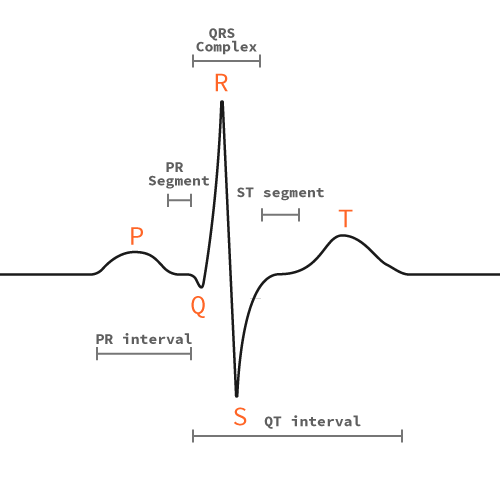
\includegraphics[scale=0.45]{img/figures/QRS.png}
\caption{QRS Complex with interval annotations}
\label{fig:qrsAnnotations}
\end{figure}


\noindent
After the leads are sampled in a wireless ECG solution, they can be streamed in raw, or compressed and optimized for transmission\cite{Balouchestani:2013dr, Alesanco:2010kc}. In order to reduce the scope of this project, we will only focus on the the core aspects of ECG. Different compression and low sampling techniques are therefore omitted completely. After being transmitted, the signals are analyzed at a processing unit, where common angles and intervals in the QRS complex as well as heart rate are calculated. The QRS complex as seen in Figure~\ref{fig:qrsAnnotations} denotes the plot or graphical representation of the electrical signals. On a per lead basis, these plots are printed on gridded paper or displayed on a monitor. Cardiologists learn to analyze the leads and are able to make a diagnosis based on different intervals in the complex, among other things. An overview of some common intervals and the different cardiac diseases they indicate are presented in Table~\ref{tab:characteristicECGintervals}. Based on this analysis, the ECG system may automatically trigger alarms if certain thresholds in the intervals are exceeded.

\begin{table}[]
\centering
\caption{Characteristic ECG intervals from \cite{Jara:2012fi}}
\label{tab:characteristicECGintervals}
\begin{tabular}{|l|l|}
\hline
\textbf{Interval QRS \textgreater 120ms} & \begin{tabular}[c]{@{}l@{}}Ventricular hypertrophy, necrosis, BCRRD,\\ BCRI, pacemakers, cardiomyopathies,  \\ electrolyte abnormalities.\end{tabular}     \\ \hline
\textbf{Interval PQ \textgreater 200ms}  & Frist-degree AV block                                                                                                                                      \\ \hline
\textbf{Interval PR \textless 120ms}     & \begin{tabular}[c]{@{}l@{}}Tachycardia, WPW, manners or \\ headphones low rates.\end{tabular}                                                              \\ \hline
\textbf{Interval QT \textgreater 450ms}  & \begin{tabular}[c]{@{}l@{}}Antiarrhytmic medicines, ischemic heart deisease, \\ cardiomyopathies, hypocalcemia, mixedema, \\ long QT syndrome\end{tabular} \\ \hline
\textbf{Interval QT \textless 350ms}     & \begin{tabular}[c]{@{}l@{}}Hypercalcemia, hyperkalemia,  early \\ repolarization, digoxin\end{tabular}                                                     \\ \hline
\end{tabular}
\end{table}

We have reviewed several earlier projects involving wireless ECG. Below we will assess one such project, while others will be discussed in~\ref{sub:bluetooth}. In Chou and Hibbs 2006 paper \cite{ChulsungPark:2006tf} they present ``An ultra-wearable, wireless low power ECG monitoring system''. They have developed and tested a contact-less ECG capacitive sensor based on insulated bio-electrodes. They imagine that these sensors can integrated into clothes, making ECG monitoring ultra-wearable. They recognize that related work based on either standard wireless interfaces or general purpose sensor nodes suffer from large form factor, low battery lifetime or low transmission speed. Because of this, their approach involve using proprietary and custom hardware in order to reach their goals. Aside from the tiny form factor, an interesting observation is their solution's power consumption, which is less than 10 mA in transmission mode and 22 mA in receiving mode. As we'll see later, this is 10-20 times the average current drawn from today's low energy sensors based on wireless standards like Bluetooth Smart. In terms of ECG, their solution support 1000 Hz sampling rate, and the analog to digital converter (ADC) is configured for 12-bit resolution. They mention their system uses 3 ECG sensors. Assuming they are referring to electrodes, and that one is for \emph{ground}, this means they can only do a 1-lead ECG. Further, they do not address any clinical aspects of their work.

% subsection electrocardiogram (end)

\subsection{Bluetooth and ambulatory ECG} % (fold)
\label{sub:bluetooth}

In accordance with our research goal of assessing available technology, Bluetooth was an attractive technology. This was because of its widespread presence\footnote{ In 2010, Bluetooth SIG estimated an annual sale of 2 billion Bluetooth enabled devices.}, as well as the low energy features introduced with version 4.0 of the specification. Bluetooth was standardized as IEEE 802.15.1, but IEEE no longer maintains the standard. The Bluetooth Special Interest Group (SIG) is comprised of more than 25,000 corporate members, which today maintain and oversees the development of the specification. There are two other IEEE 802.15 standards discussed in relevant literature, namely 802.15.4 and 802.15.6. The first one is likely to play a significant role in the development of future IoT applications.\footnote{ See Google's Thread protocol and Zigbee for implementations of this standard.} As the second one is still in development, this thesis has not assessed the work on 802.15.6. However, of these standards and their implementations, Bluetooth is the most available today. In this section we will cover the basics of Bluetooth Smart and discuss related research projects using the technology in combination with ECG monitoring.

\subsubsection{Bluetooth Smart} % (fold)
\label{ssub:bluetooth}

Bluetooth originated from Ericsson in 1994, and has it's name from a Danish/Norwegian viking king that was characterized as a ``good communicator''. Since it's origin, the standard has seen 4 major releases, and several minor ones.\footnote{ The latest of which (4.2) was released in December 2014} The next big release, version 5.0 is currently being being drafted, and is expected to be formally announced later this year. 

Version 4.0 introduced new low energy features, which was originally branded with the suffix ``LE'' or ``Low Energy''. Because of confusion around the ``low energy'' devices and those implementing older versions of the standard, Bluetooth SIG announced their new branding strategy in 2011. The new logo and name read \textit{Bluetooth Smart}. Throughout this thesis we will focus exclusively on the low energy features of the standard and we believe the suffix ``low energy'' is less ambiguous than ``Smart''. Because of this we will be using both the old and new name based on what's most describing.

% subsubsection bluetooth (end)

\subsubsection{GATT and Profiles} % (fold)
\label{ssub:gatt_and_profiles}

The Bluetooth standard specifies a series of communication protocols that together constitute the complete Bluetooth stack. This stack is separated in two; the \emph{Host} and \emph{Controller}. The controller stack is concerned with the lower network layers and is usually implemented in the firmware of silicon devices containing a Bluetooth radio. The host stack are upper layers, and is usually implemented as part of a operating system and runs on a processor together with the user application. With resource constrained devices such as those we'll investigate in this thesis, both the controller and host can be bundled together. They will then run on the same microprocessor, making up what is known as a ``hostless'' system. See Figure~\ref{fig:bleNordicHost}. 


\begin{figure}[H]
\centering
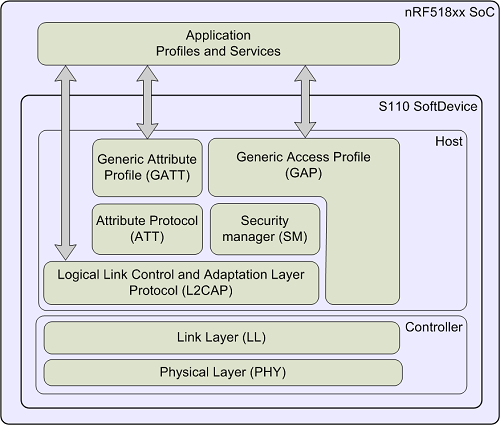
\includegraphics[scale=.8]{img/figures/bleNordicHost.png}
\caption{Overview of the Bluetooth protocol stack on a hostess system~\cite{nordicSDK}}
\label{fig:bleNordicHost}
\end{figure}


% TODO wite about advertising, connection establishment? roles (master and slave / initiator advertisor)
\noindent
In this thesis we are most concerned with the higher layer protocols, more specifically the GATT profiles. This is an acronym for Generic Attribute Profile, and it is responsible for ensuring interoperability in data exchange between two two Bluetooth devices. The profile defines the types of state data that a device exposes and how that data can be used. Profiles are organized in services, which contain one or more characteristics and descriptors. The profiles and its characteristics are specified by working groups within Bluetooth SIG. The process of how these are developed and implemented are discussed in Section~\ref{sub:interoperability}. More information about how connections are established and data is transmitted, can be found in Section~\ref{ssub:maximum_throughput}.

% subsubsection gatt_and_profiles (end)

\subsubsection{Bluetooth enabled ambulatory ECG} % (fold)
\label{ssub:bluetooth_enabled_ambulatory_ecg}

We have reviewed multiple previous research projects evaluating Bluetooth Low energy as a wireless technology for streaming ECG data. In this section we will review two of them.

Jara et at. evaluated Bluetooth low energy as a technology for streaming continuous data from a wearable ECG in their 2012 paper. Similarly to our project, they focused on analyzing the capabilities of Bluetooth Low Energy as a medium for streaming raw ECG data. Their initial evaluation concluded that it was necessary to compress the ECG signals before transmission. They built a prototype based on a Bluegiga development kit. This development kit comes with its own Bluetooth API, built on top of the Bluetooth stack, which is programmable with a language called BG-script. They do not mention the amount of leads simulated, and their calculations are hard to follow. For their experiments, they operated with a ECG sampling rate of 300 samples/second. We were unable to recompute their calculated throughput, but they conclude that Bluetooth Low Energy in 2012 is not well suited for raw ECG transmission. However, a lot has happened with the specification since then.

Another paper describing ECG data transmission with Bluetooth Low Energy (BLE) is \cite{Anonymous:1SQ78ejy}. They built a three tier of 2 development kits and an Android application. This paper is from 2013, at which time Android did not fully support low energy Bluetooth through their SDK. Because of this, their system is comprised of 3 parts, one low energy board with a Bluetooth interface, one ``converter'' board, that speaks both BLE and Bluetooth 2.1. This board is responsible for proxying the data from the sensor board through to the Android application via Bluetooth 2.1. At the sensor board, they developed a ECG patch system, which records ECG through by using 4 electrodes. They operate with a maximum data rate of 306 kbit/s over the BLE connection, and they claim ECG has to be sampled with at least 250 samples/s. Finally, of interest to this project, they did some preliminary battery tests, and concluded that the batteries lasted between 9 and 13 hours depending on the surrounding temperature.

Other literature related to ECG and its clinical requirements is discussed further in Section~\ref{sub:evaluation}. One common denominator through the review of these and other research projects, is that no one seems to agree on what's the required sampling rate for ECG, and the size of each sample should be. Further we recognize that very few, includes the clinical aspects and use cases of doing ECG.

%  93 papers reduced to 39 reduced to 5

% subsubsection bluetooth_enabled_ambulatory_ecg (end)

% subsection bluetooth (end)

\subsection{Wireless Body Area Networks} % (fold)
\label{sub:wireless_body_area_networks}

% \subsection{Wireless Body Area Networks} % (fold)
% \label{sub:wireless_body_area_networks}

% The notion of a mobile gateway has been widely adopted and discussed \cite{Movassaghi:2014hi, Mohammed:2014dw, Touati:2015gy, EmilJovanov:2005ty} in earlier research.
% Missing.
% TODO mention the differnt classes of prioritized data

% TODO Mention 802.15.6

% subsection wireless_body_area_networks (end)

A lot of work has been done within the field of Wireless Body Area Networks (WBAN). This is a truly multidisciplinary field, that is concerned with everything from antenna design and MAC protocols and smart temperature-based routing schemes \cite{Movassaghi:2014hi}, to hospital, clinical and medical topics ranging from infrastructure to cardiac arrhythmias. In our case we were not very much interested in the actual networks, as much we were in the problems faced in both the development of WBAN and using low energy sensors for physiological monitoring. Because of this, we have researched a lot of different WBAN problems, in order to find the problems that had already been solved, that might benefit us. In terms of architecture, and the organization of devices outside and around the WBAN, we have investigated several approaches. In the following section some of them will be discussed.

Previous research have proposed categorizing WBAN data in different tiers, based on clinical priority. A real-time ECG stream may be of higher clinical value and have higher QoS requirements than the occasional temperature measurement.\footnote{ Note that deep Vein Thrombosis, or blood clots, can be detected by sudden temperature changes in extremities.}.

A fundamental question in WBAN how to implement the gateway. Most research uses a gateway of some sort, and different solutions to how to connect a WBAN to external devices and services has been proposed\cite{Shahamabadi:2013df}, some more controversial than others \cite{Zachariah:2015cm}. Most of the architectures we reviewed involve a personal server, or personal gateway as we refer to throughout this thesis. The role of this gateway and it's capabilities define in many ways how the rest of the infrastructure is going to look like. Shahamabadi et. al. presents a good overview of the most reasonable ways of organizing this in \cite{Shahamabadi:2013df}. Here they present a solution to support mobility in . They present 3 different combinations: One where WBAN nodes communicate directly with a boarder router, i.e. without a personal gateway (or mobile router as they call it), another one where all traffic from the WBAN is routed through a personal gateway, and a hybrid of the first two.

The last approach involves using mobile gateway just as a facilitator for ``administrative'' tasks like coordinating access point handoff and roaming on behalf of the WBAN. This solution require that the WBAN sensors send physiological data directly to a smart access point. This proposition solves the problem of the mobile gateway becoming a bottleneck because data does not have to be routed through the gateway. A smart access point would also have more resources for doing intermediate data-processing~\cite{DrAmirMohammadRahmani:2014vx}. However, there is no silver bullet, as this has approach involve a higher energy consumption: With this organization the node antennas would have to consume more energy in order to send data directly to an access point or border router which would typically be located further away than the mobile gateway. 

However there are tradeoffs with all solutions. Making a single gateway the sink of several sensors organized in a WBAN creates a single point of failure. With a single point of failure, ensuring the personal gateway is working properly will become of outmost importance, as a faulty gateway will not only take down the low priority sensor measurements, but also the critical ones. As we'll see in later sections, today's telemetry solutions operate with zero downtime.

% subsection sub_wireless_body_area_networks (end)

\subsection{Interoperability} % (fold)
\label{sub:interoperability}

Rahmani et. al. gives a clear overview of different forms of interoperability in their 2015 paper about Smart e-Health Gateways~\cite{DrAmirMohammadRahmani:2014vx}. They separate the concern of interoperability and reconfigurability into the following categories: Device interoperability, protocol interoperability, data interoperability, reconfigurability and device discovery and mobility support. In the following sections we will give an overview of data interoperability related to Bluetooth.

\subsubsection{Data Interoperability} % (fold)
\label{ssub:data_interoperability}

% subsubsection data_interoperability (end)

Document and message standardization in health care is a huge topic and certain actors like HL7 have been working actively with standardization development for the least 30 years. In this section we will cover WBAN related papers discussing interoperability as well as giving an brief overview of the latest standardization efforts made by actors like HL7, Continua and the Bluetooth SIG.

The Continua Alliance develops interoperability guidelines and offer device manufacturers a way of certifying their Bluetooth Smart devices for Personal Connected Health. Their guidelines are globally recognized as the only standard for Personal Connected Health \cite{newRef:27}. The certification program is organized as follows: Continua selects and approves certain GATT Profiles (aka. Smart Profiles). Devices that support these profiles can be certified, meaning that they will be compliant and that the data they deliver can be ``mapped into the Continua & HL7 Record-set and shared, where it can become available as needed to social media, care providers, hospitals, clinicians, etc.'' \cite{newRef:27}.

How are Bluetooth Smart profiles implemented? Efforts are being made by Bluetooth SIG to standardize data profiles in order to ensure interoperability between devices supporting the protocol. A profile for a type of device defines the GATT Services which a device of this type must or may implement. The GATT profiles are specified by the Bluetooth SIG through Device Data Specifications. This work is organized in different domains and there is a specific sub-group for Health Device Profiles (HDP) (current version 1.1), some of whom are approved by Continua. HDP defines devices as either sinks or sources. In this thesis these roles are referred to as as nodes and personal mobile gateways.

The HDP specification does not specify the format nor content transmitted, but confine to ISO/IEEE 11073-20601 Personal Health Data Exchange Protocol \cite{newRef:18}. Bluetooth SIG require devices implementing the HDP to follow the ISO standard for exchanging data between HDP devices and IEE 11073-104xx Device Specification. However, from ISO/IEEE 11073-20601 Data Exchange Specification, ISO/IEEE draws a clear line between consumer electronics and medical devices: 

\begin{quote}

\textit{``Provides strong application level interoperability by operating with the ISO/IEEE 11073-20601 Personal Health Data Exchange Protocol [7], which defines a transport-agnostic Data Exchange Protocol and representation of device application data based on international standards. This standard defines a common core of communication functionality for personal telehealth basic ECG (1- to 3-lead ECG) devices. Monitoring ECG devices are distinguished from diagnostic ECG equipment with respect to including support for wearable ECG devices, limiting the number of leads supported by the equipment to three, and not requiring the capability of annotating or analyzing the detected electrical activity to determine known cardiac phenomena. This standard is consistent with the base framework and allows multifunction implementations by following multiple device specializations (e.g., ECG and respiration rate).''} \cite{newRef:18}

\end{quote}

% The Health Device Profile specification mention ECG as an example of data transmitted on Streaming Data Channels,


% subsection interoperability (end)

% section section_name (end)
\section{Research Strategies} % (fold)
\label{sec:method}

The most critical success factors in every research project lies in the researcher's ability to plan, execute an monitor the study. A clear research strategy needs to be clearly defined, revised and followed. This chapter will lay out the research strategy applied in this project, and discuss how we approached the different research stages.

\subsection{Research Methods} % (fold)
\label{sub:research_methods}

Wireless monitoring of physiological metrics is a wide topic covering many similar or related instances of the same problem. In order to reduce the scope we decided to look at only one instance, namely wireless ECG monitoring. Because of this, the project in it self can be considered a case study in ECG. It was important to us that we investigated ECG in depth, as well as studying the practice in it's natural, clinical setting. This is reflected in our data collection methods, which include multiple sources and methods and has a focus on relationships and processes.

Like in any project involving people and technology there is an inherent complexity that the researchers have to unravel in order to understand the forces that guide the socio-technical systems in front of them. We want to avoid the deterministic approach of attributing properties to technology that guarantee the effects and outcome it will have on health care. For this research project it was clear that we needed to approach the practical clinical aspects in addition to the technical aspects of ECG monitoring. Different stakeholders may have different views and knowledge about various aspects of the challenges with todays monitoring systems. In order to achieve a deeper understanding of the context and difficulties, we decided to approach both medical professionals and technical engineers. Because of this, we differentiate our data collection methods in those applied when researching the technical side of these systems, and those applied when exploring the medical domain and current practices.\\
\newline
\noindent
\textbf{Clinical:} In order to understand how and why ECG monitoring is practiced, we applied mainly qualitative techniques. This was done through observations and interviews with medical professionals, and will be discussed further in Section~\ref{ssub:interviews} and Chapter \ref{sec:clinical_context}.\\
\newline
\noindent
\textbf{Technical:} Our strategy for researching the technical requirements to clinical ECG monitoring systems involved understanding both today's existing technical solutions and those proposed in literature. Because this a wide field spanning different domains, several methods for data collection have been utilized. These include interviews, document and literature analysis, and experiments, as discussed further in Section~\ref{sec:experiments} and Chapter~\ref{sec:technology_assessment}.
\\
\newline
\noindent
When studying these systems it is important to understand why and how an prototype works in it's environment, not only that it works. Our overall approach have been influenced by both the Design Science methodology, the research team's personal experiences and IBM's framework for Design Thinking \cite{ibmDesignThinking}. The latter embrace a iterative strategy for understanding peoples contextual needs and deliver outcomes. This neatly ties together our study of clinical practices with the technical research:

\begin{figure}[H]
\centering
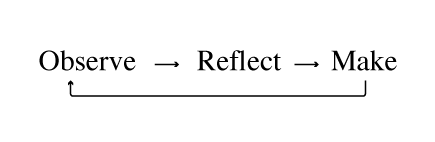
\includegraphics[scale=0.6]{img/figures/designThinking.png}
\caption{From IBMs Design Thinking framework}
\label{fig:ibmDesignThinking}
\end{figure}

\subsection{Interviews and observations} % (fold)
\label{sub:interviews}

% subsection interviews (end)
This section will describe interviews, how they were conducted and the inherent strengths and weaknesses of doing interviews.

In order assess the validity of our observations and get multiple sources, we decided to conduct interviews at two different Norwegian hospitals. This way we could either record the differences in ECG monitoring practices or confirm that they were the same. Norwegian hospitals are usually organized with an in-house department for technical engineers, which made it easier for us to organize the interviews with different stakeholders.

A lot of knowledge is embedded in the people and practices of their every day routines. An introductory conversation at the first hospital revealed that nurses at both the intensive care units and the cardiac observation unit had most practical experience with the technology. In these units they handle ECG and telemetry solutions on a daily basis. After this quick survey we constructed both unstructured and semi-structured interviews for both hospitals with a focus on open questions. This way we were able to develop a understanding of how people viewed their work and how they interpreted the technology that was part of their everyday routines. This also made the research more flexible, as we were able to do interviews with nurses in their natural working environment on a short notice.

We also arranged for two observation sessions at the second hospital, in order to see for ourself how different aspects of patient monitoring were carried out. In the first session we observed a nurse preparing and conducting a full 12-lead ECG test on a colleague, and in the second session we observed another nurse monitoring 10 remote telemetry patients, and 6 bedside patients in a intensive care unit. During both observations, we got the chance to ask follow-up questions, which further increased our understanding.

Although nurses have most practical experience with the monitoring practices, they do not assess the ECG plots diagnostically. Because of this we also conducted two semi-structured interviews, with a cardiovascular surgeon and an anesthesiologist. These interviews were conducted later in the project and provided clarifications, useful diagnostic insight as well as domain knowledge.

Because this is a highly specialized field, most knowledge is embedded in the workplace. This also holds for the technical knowledge. In order to learn about the technical solutions backing the ECG monitoring we reached out to the clinical engineers at both hospitals. Conducting structured interviews was inexpedient in the beginning, and we began with unstructured interviews at the first hospital. After we had established a basic understanding of the components and solutions, we moved on to conduct semi-structured interviews at the second hospital. This enabled comparison of the technical solutions between the two hostpial.

As mentioned in Chapter~\ref{sec:literature_review}, wireless body area networks and sensor technology are active research areas. In order to gain valuable insight in this development we conducted another unstructured interview with a researcher working with short-range wireless monitoring in critical care at The Intervention Centre at Oslo University Hospital.

All in all we conducted 8 different interview sessions, talking to a total of 10 people. This included 4 clinical engineers, 3 nurses, 2 physicians as well as the clinical researcher from The Intervention Centre. During all interviews we took note of people's experience with, interpretations of, and reactions to the technical monitoring systems and daily routines. We observed what people said and did, and afterwards reflected over what they did not say or do. This way we were able to search for latent needs in the existing practices. The knowledge gained from these interviews are treated in  Section~\ref{sec:clinical_context}.

% subsubsection interviews (end)

\subsection{Experiments} % (fold)
\label{sub:experiments}

% TODO Wirite about how we want to make a protoype 
% TODO Skriv om begresninger ved prototypen

In order to answer our problem statement and main research question, we wanted to build a working prototype based on available technology and open standards. The prototype was validated through experiments, testing certain critical aspects of ECG based on the knowledge gained throughout the project. These experiments can be found in Subsection~\ref{sub:evaluation}. We wanted to test if these minimum requirements could be upheld, and did not exceed the requirements required for clinical use.

% subsection experiments (end)


\subsection{Document and literature analysis} % (fold)
\label{sub:document_and_literature_analysis}

A lot of work has been done within the field of WBANs and telemetry, and a systematic approach to gathering, analyzing and extracting knowledge from previous work was an absolute necessity. This section will describe how we collected literature and documents from previous research and existing solutions to investigating the topic of WBANs.

Searching for information was a maturing process. Finding the right search terms did take some time, but we found the most relevant results on Google Scholar using a combination of keywords such as \textit{``WBAN, WSN, patient monitoring, BLE, Bluetooth Smart, ambulatory patient monitoring, ECG, Ubiquitous Healthcare''}.

Documents were collected from two sources: The Norwegian Directorate for e-Health supplied us with standardization documents and guidelines from Continua Health Alliance. These are documents describing interoperability aspects such as how data should be exchanged between sensors, gateways and end services. We received in total 8 documents in the H.810-813 series, dated 2014. One of the clinical engineers also supplied us with installation and service manuals to the telemetry system they had installed. This were 2 documents and one presentation dated 2007, describing the Philips IntelliVue telemetry system in detail.

% subsection document_and_literature_analysis (end)

% section method (end)
\section{Clinical Context} % (fold)
\label{sec:clinical_context}

This section describes our findings from the interview sessions. These findings form the basis of our use cases as well as some functional requirements. We will discuss both similarities and differences found in clinical practices as well as describing the patient monitoring solutions deployed today. Throughout this section we will refer to the three most important stakeholders, which is listed below:

\begin{itemize}

  \item[\textbf{Patients}] The patients themselves are the main source of physiological data. The patients are the ones in direct contact with the sensory equipment, and will act as the wearer of the  WBANs. It is important to remember that these are people admitted to the hospital with a broad span of medical conditions. They might be in pain, unconscious, or mentally exhausted. One must take these considerations into the design and requirement specification.
  
  \item[\textbf{Practitioner}] We define health practitioners and clinicians are the medical staff that are responsible for care and treatment of patients, as well as operating their respective wards, departments or units. They are the ones that will install the sensors on the patient, and monitor the signal as they arrive at the central.

  \item[\textbf{Clinical Engineer}] Clinical engineer is defined as the medical and biomedical maintenance engineer responsible for installing and maintaining the technical equipment used for medical purposes at hospitals. Among other things, they are responsible for doing technical maintenance on the central heart monitoring system, which is as close as we come to an established way of monitoring vital signs wirelessly of multiple patients in hospitals today.

\end{itemize}

The rest of this chapter will be organized as follows: 
We will end this chapter with a detailed overview of different use cases.

\subsection{Intended use} % (fold)
\label{sub:intended_use}

The researcher from The Intervention Centre made it clear that we had to consider the intended use for our prototype. Monitoring ambulatory patients is merely an action following an intention, not the goal in itself. Therefore we must ask, for what patients are we developing this solution? What use-cases? What is the intended use?

Before we answer these questions, a little introduction to cardiac patients and patient monitoring in practice is needed. Most patients in a hospital today are not electronically monitored on a daily basis. There are however certain units in a hospital that monitor patients continuously. In the Intensive Care Unit (ICU) as well as the Postoperative Unit (PO) all patients are monitored (ECG, SpO2 etc.) around the clock regardless of their diagnosis. The same accounts for Heart failure Units (HFU) and Intermediate Care Units (IMC) which are wards for patients with cardiac conditions and intravenous medications that require continuous cardiac monitoring and treatment. Depending on the hospital it may have one, two or all four units. All these units usually holds patients temporary before and after a surgical procedure or intervention - here meaning catheter based non-surgical procedures. When asking the cardiovascular surgeon about common heart disease diagnoses at these units, he said the following: 

\begin{quote} 
\textit{``Acute Coronary Syndrome (ACS) is a group of conditions related to a decreased blood flow in the arteries to the heart, also known as the coronary arteries, resulting a “myocardial ischemia”. This cause a shortage og oxygen and glucose needed for cellular metabolism and makes the heart muscle unable to contract properly and in worst case it will die. This is called a myocardial infarction, better known as a “heart attack”. These coronary artery diseases are the most common cause of death globally. Typically for all ACSs is that they are often diagnosed by ECG. Patient having an ACS needs a continuous monitoring before, during and after therapy, sometimes for days and sometimes even for weeks. Patients at the IMC, or those transferred to normal wards and to  rehabilitation may still suffer from different consequences after a myocardial infarction like cardiac arrhythmias and even new cardiac ischemia.''}
\end{quote}
\noindent
This is the reason why patients at risk are fitted with a telemetry in order to be monitored. The clinician(s) at a monitoring central observes the heart rhythm and looks for signs of unusual elevations or interval variations in the QRST complex. See Table~\ref{tab:table_heart_irregularities}. Abnormalities above or below a given threshold often generate alarm triggering events. The thresholds comes with a default setting and is customizable per patient in the monitoring central. 

There is typically one such monitoring central at a given hospital. But where it is located varies. At the first hostpial we visited, the central monitoring capability was located in a dedicated HFU. The second hospital didn't have a dedicated HFU, and the central monitoring station was located at the intensive care unit. 

Based on the observations above we define the intended use for this system as follows:

\begin{quote}
\textbf{Intended use:} To remotely monitor not critically ill patients at risk for complications regarding an acute coronary syndrome (susceptible for heart defects), located at an IMC or in another ward.
\end{quote}
\noindent
In other words, the intended use is on patients that would have been equipped with a telemetry device today. The existing systems are used for monitoring patients that are expected to experience, or are vulnerable to, heart defects either pre or post surgery, or during treatment. See table Table~\ref{tab:table_heart_irregularities} for a description of the most common irregularities and how they are identified. Because irregularities can happen at any time of the day and night, continuous monitoring is a fundamental requirement to the prototype.

% TODO insert fig:10_leadECG
% TODO Insert fig:pappa_ecg
% TODO Insert table_heart_irregularities

% subsection intended_use (end)

\subsection{Existing Solutions} % (fold)
\label{sub:existing_solutions}

Interviews with medical engineers at both hospitals revealed that both had a telemetry system from Philips installed. In both cases the network infrastructure and equipment was produced by Philips, but was delivered and maintained by different local partners. This section will describe the IntelliVue telemetry system from Philips, which as we found out, is deployed at several Norwegian hospitals today. The studying these systems were conducted in order to gain insight in the practice of wireless patient monitoring today, as well as giving us an indication of how prepared hospitals are for WBANs from a infrastructural point of view.

\subsubsection{System Architecture} % (fold)
\label{ssub:system_architecture}

The Philips IntelliVue telemetry system is a complete end-to-end system enabling both wired and wireless monitoring of ECG. For the medical practitioners the system is composed of two components: the TRx4841/51A wireless transceivers and the IntelliVue Information Centre. The TRx transceivers are devices for capturing ECG and SpO2 on adult and pediatric patients, and are worn by the patients. Powered by two AA batteries they  capture and stream a 3 or 5 lead ECG to a custom 802.11 type access point (AP) operating in the 2,4 GHz spectrum. These APs are installed in addition to, and independent of existing public or private WiFi access points. Because Philips provide all hardware in this closed system, the telemetry system does not have to confine to the interoperability requirements it would needed if the system were to allow for proprietary sensors and measuring devices. The wireless interface does not strictly follow the 802.11 specification, and the system offer a ``Smart Hopping'' technology in order to reduce collisions on the already crowded 2,4 GHz network band. This is made possible by synchronizing all access points through a dedicated sync unit. Another noteworthy network feature is the ``make before break'' method that improves the roaming abilities. The TRx transceivers will look for new, stronger access points when they detect a decay in signal strength with the current AP. The system will make sure to connect transceivers to the new (stronger) AP before breaking with the previous one, enabling a more reliable handoff between access points. The network coverage at the second hospital were almost 100\%, while the first, larger hospital offered 100\% network coverage in one of it's buildings.

As mentioned, this being a end to end system the IntelliVue patient monitoring suite includes everything from transceivers, bedside monitors, access points, routers, gateways, network switches, uninterruptible power supplies (UPS), processing units and databases in addition to the optional printer Figure~\ref{fig:intellivue_telemetry_architecture}.

% TODO Insert fig:intellivue_telemetry_architecture

Offering every piece in this architecture enables Philips and its local distributers/providers to guarantee good QoS metrics which is essential for wireless patient monitoring applications. However, installing a complete system like this comes with a substantial cost, and ties you down to just one provider for an extended period of time. The IntelliVue Telemetry system at the first hospital was installed in 2009, and is expected to have a lifespan of at least 10 years. This reduces the flexibility and ability to adapt new solutions. On the upside, an all-in-one solution like can easier guarantee QoS as well as offering better support and maintenance. It's easy to think that this also might reduce the need for interoperability - because Philips controls the whole stack. Having studied the solution being used in practice, we would argue this is false. An example of this can be found in the installation of the CorPulse ECG device from Alere \cite{alere}. This is a device installed in emergency vehicles enabling a short, pre-hospital ECG to be sent via a SIM card and the 3G network. This is often critical information that enable the medical staff to make informed decisions before the patient arrives at the hospital. Because this is a different system from a different provider, the hospitals we visited had installed a standalone computer next to the central monitoring information center system from Philips. This standalone computer display the pre-hospital ECG from the Alere device. Although coming from a different source, having a standalone system for viewing ECG next to a central ECG monitoring solution is suboptimal. Suboptimal not only in technical terms and with regards to maintenance, but also from a user experience point of view. The lack of integrations creates yet another technical dependency in the everyday life of medical practitioners. One consequence of \emph{inoperable} devices can be seen in Figure~\ref{fig:bilde_av_alere_ecg}. A workaround for dealing with separate systems is sharing login credentials, which render the security measure completely useless. Based on these observations, we believe interoperable devices and services will be crucial for the success of a ubiquitous health care.

% subsubsection system_architecture (end)

\subsubsection{The Transceivers} % (fold)
\label{ssub:the_transceivers}

The TRx transceivers are small and lightweight with a limited user interface. It was reported they have a battery lifetime a little over 24 hours, which fits well with the number found in the user manual (up to 48 hours). As we'll see in Section~\ref{ssub:maximum_throughput}, the average throughput is tied to sampling rate. In order to establish a standard for what throughput wireless ECG must support we reviewed both literature and the user manuals for the IntelliVue Telemetry system. As the numbers used in literature varies a lot, we searched the transceivers for this information. However, we were unable to find any information about neither the sampling rate nor average throughput the transceivers delivered. Both Philips and the local providers of the system were consulted, but no one could give us a clear answer. When this failed, attempts were made to find the information based on network traffic, but we never got hold of the telemetry network administrator.

Although the IntelliVue wireless transceivers provide ambulatory and bedside patient monitoring, there's a catch with increasing the mobility other than the movements themselves. Usually when doing a detailed 12-lead ECG, medical practitioners place the 4 extremity electrodes at the wrists ankles. In telemetry these electrodes are often moved to shoulders and hips in order to increase mobility. However, because of the large muscle mass located in these areas, the recorded ECG signal is prone to more muscle noise. We observed this ourself while studying a 5-lead telemetry reading at one of the hospitals. Accurate, unobtrusive and noise resilient sensors like the ones in \cite{ChulsungPark:2006tf, Anonymous:FtVb5yQr} will be an absolute necessity in persuasive patient monitoring. 
\\
\newline
(...)
\\
\newline
Unlike multimedia streams, a physiological data stream cannot be buffered to mask jitter and latency on the receiving end. End to end latency will therefore be experienced as gaps in the monitoring stream, thereby invalidating the purpose of the system.

% TODO Insert this somewhere

\footnote{It's worth noting however that a decision support system based on data mining would usually not have the same real-time requirements and would not suffer from potential latency}

% subsubsection the_transceivers (end)

\subsubsection{The Information Centre} % (fold)
\label{ssub:the_information_centre}

The information center can provide a web view for accessing the patient data from outside the monitoring central. According to the service manuals they claim that the information displayed in the web view should be near-real time with little delay, but recommend users to always use the bedside monitor or the information center for real-time monitoring. We were unable to find a accurate metric for the end-to-end latency in IntelliVue's documentation. However, because the providers have full control over the whole infrastructure and the distances at a hospital are relatively small, it is reasonable to assume this delay is less than 2 seconds from the measurement to the information center.

An alternative approach to getting information about acceptable transmission delay would be to measure the actual network traffic in the systems deployed today. However, we were unsuccessful in getting in touch with the network administrator at either hospitals.

Information on transmission delay is also scarce in the literature we reviewed. Within the field of WBAN very few address this issue, and and we had to look into Telemedicine in order to find any suggestions to end to end latency at all. Through clinical trails, Alesanco and Garcia suggest 4 seconds as the maximum acceptable delay for a reliable real-time ECG transmission. Their research however is concerned with telemedicine over 2G/3G networks, and the intended use and QoS are different. This being the only exact metric we could relate to, we chose to use this as our baseline for network delay.

% subsubsection the_information_centre (end)

\subsubsection{Other ECG devices} % (fold)
\label{ssub:other_ecg_devices}

If there was something suspicious with the readings on the screen, both the ICU and the unit with the remote patients had several standalone 12-lead ECG units that could be connected to the patient on request. We observed how a patient could be connected to the standalone ECG device with 10 electrodes in order to get the full 12-lead resolution. This device was mobile (on wheels) and had the form factor of a small laptop computer. See Figure~\ref{fig:10_leadECG}. It was standalone in the sense that it's only output was a printed exert from the examination as shown in Figure~\ref{fig:pappa_ecg} from a built in printer. We also visited two other medical units at the same hospital that did ECG monitoring. Both of which used a 3-lead setup. This stands to show that at the second hospital, 3 and 5-lead setups are most used in continuous monitoring. The full 12-lead was only used in short examinations on demand. This practice was also confirmed at the Clinic of Cardiology at the first hospital.


% subsubsection other_ecg_devices (end)

\subsection{Use Cases} % (fold)
\label{ssub:use_cases}

One limitation of previous research is the lack of practical use cases. We believe these has to be included in order to get an understanding of the context the solution have to support. The following use cases are related to the technical and mobility aspects of the monitoring solution. Keep in mind that these use cases only assess some parts of the system.

\newline
\noindent
\textbf{Patient}

\begin{enumerate}

  \item[\textsc{U1.1}:]\textbf{Stationary:} This use case will describe the situation where a patients monitored while lying in bed. Here both gateway and sensor would be stationary.

  \item[\textsc{U1.2}:]\textbf{Partly ambulatory:} Here patients are monitored while walking around their bed. This means the patient is ambulatory while the gateway is stationary.

  \item[\textsc{U1.3}:]\textbf{Ambulatory:} This use case describe the situation where patients are monitored while walking around the room or ward, with the personal gateway in their pocket. This means the patient is fully ambulatory.

\end{enumerate}

\newline
\noindent
\textbf{Medical Professional}
\begin{enumerate}

  \item[\textsc{U2.1}:] Setting up the patients personal gateway
  \item[\textsc{U2.2}:] Monitor a patients ECG on a separate device

\end{enumerate}

% section clinical_context (end)
\section{Technology Assessment} % (fold)
\label{sec:technology_assessment}

According to the four types of prototypes in design science \cite{Johannesson:2014co}, our artifact was intended to be of the model type. A model can be used for supporting the construction of other prototypes, and hopefully our model can be reused by later projects. We wanted to come up with a design and then create a prototype that let us test different aspects of using low energy sensors for wireless ECG monitoring. Based on what we knew from previous literature we decided the following three aspects constituted the baseline functional tests that would answer our research questions:
\begin{itemize}
	
	\item End to end latency
	\item Battery life
	\item Maximum throughput
  
\end{itemize}
\noindent
We validate our proposed design through a working prototype. Our prototype takes the form of a test bed that can be used to address the items listed above experimentally. This section starts with a discussion on different technical and architectural alternatives, and the decisions that went into it. Later we describe how the base of the testbed was implemented, before we customized it in order to evaluate the baseline functional tests.

\subsection{System architecture} % (fold)
\label{sub:system_architecture}

As mentioned in Section~\ref{sec:literature_review}, different architectures has been proposed and discussed in large by previous research. A general solution to how WBANs should be organized in relation to existing infrastructure do not exist, and is an important research topic. Mainly two different architectures have been discussed earlier: One where the WBAN routes all traffic through a personal gateway, and another one where it directs the traffic directly to an access point. See Figure~\ref{fig:architecture}. In \cite{Shahamabadi:2013df} a third approach is proposed. This merges the two former ones, where WBAN data is sent directly to the access point, while the personal gateway is given the responsibility of coordinating mobility issues like exchanging handover messages on behalf of the WBAN. In the following section, we will compare the first two approaches as seen in Figure~\ref{fig:architecture}.

\begin{figure}[H]
\centering
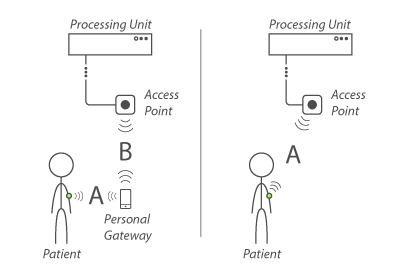
\includegraphics[scale=0.75]{img/figures/architecture.png}
\caption{Here A represents Bluetooth Smart while B is 802.11}
\label{fig:architecture}
\end{figure}

\noindent
Based on what we know about the existing telemetry systems deployed today and the research on WBAN sensor devices, it is improbable that all sensory devices will be (A) developed by the same manufacturer, and (B) that they all communicate over the same physical medium. The question of data interoperability is an interesting topic, because of the technical constraints imposed by the small sensors. At what point in the pipeline do we enforce the standardized data formats for exchanging medical information? In general, we believe this should be done as early as possible in the process, preferably at the node level. However, we want to highlight two arguments to why this might not be optimal: Although there has been invested a lot of effort by standardization organizations like HL7 and OpenEHR the last 30 years, data standardization in health care remains a challenge - not only across institutions, but also between information systems located at the same hospital. Based on this, requiring standardized formats with reduced footprint, optimized for constrained sensory devices, might not be realistic. As mentioned in Sect. 3, organizations like Continua are currently trying to bridge this gap, but with a primary focus on personal health technology, not clinical. This is a topic that need more research.

Another argument to why it might not be feasible to enforce todays standardized data formats for physiological measurements at node level, is related to the technical constraints of these devices. In order to keep the energy consumption down, overhead is reduced and as little data as possible is sent. This is especially true for continuous, streaming data sources like ECG. The approach Continua and ISO/IEEE has to this problem is to make smaller standardized measurement data formats tailored for constrained devices. Then they specify how these data formats should be transformed or mapped onto richer, data formats with a larger space footprint at a gateway level.

Relating this to the architectures discussed in previous research, we identify certain practical advantages of routing all traffic trough the personal gateway: Making a personal gateway compatible with a given sensor and its manufacturer specific or protocol specific\footnote{If standardized data formats are used} data format is a trivial task through software applications installed on the personal gateway device. The same triviality does not hold for a smart access point/boarder router wanting to transform the data into a richer, standardized data format. In a reality where a standardized data format is not implemented by every sensor node, giving an access point the role as a WBAN sink, as suggested by \cite{DrAmirMohammadRahmani:2014vx} seems highly impractical: All access points in a roaming environment would have to be compatible with custom data formats from several WBAN sensors carried by a multitude of patients. In this scenario, we only see smart gateways/access points being able to fulfill this data processing and transformation responsibility if standardized data formats for every physiological measurement is implemented at WBAN node level.

Based on these considerations, our proposed architecture consist of the following parts: a single sensor node simulating a patient ECG device, a personal mobile gateway acting as a WBAN sink to be carried by the patient, a monitoring server available on a local or remote network together with a client interface for remote monitoring. In order to reduce the scope and complexity we have decided to only include one node in our prototype. This is a clear limitation with our prototype and study, as we only consider a single-hop star network topology in instead of a mesh topology, which is proven to be the most effective topology for WBANs. One concern here might be that Bluetooth does not currently support mesh networks, but as as Feb. 24 2015 the Bluetooth SIG formally announced formation of the Bluetooth Smart Mesh Working Group \cite{bt:sig:mesh}, and we operate under the assumption that this will be supported in future versions. The gateway should have the responsibility of routing the sampled data from the WBAN to an external endpoint. In accordance with Continua's guidelines, we also propose that the gateway enforce interoperability by transforming the data into a standardized medical format. But how can this be accomplished in a multi sensor, multi manufacturer environment? 

We believe this can be solved by using the repository architectural pattern. The gateway application could be extendable with different ``profiles'' to accommodate for both different manufacturers,  different communication protocols, and different data formats. These profiles would be installed from a repository, central to a hostpial, region or country depending on the supported data formats. The profiles would contain a mapping between a given sensor peripheral and the preferred output data format compliant with the monitoring system a given hostpial was using. This way, the hospital could support a growing amount of sensor peripherals, independent of sensor manufacturer.

See Table~\ref{tab:system_components} for a formal description of each component of our prototype.

% TODO create table system_components

An overview of the different prototype components:
\begin{itemize}

  \item[\textbf{Node:}] A node is the sensory device that does one or more physiological measurements and communicates it wirelessly to either another node or to a sink in the WBAN. In order to achieve wearability the nodes has to be as small as possible. Batteries are often the largest part of today’s sensory nodes and the biggest energy consumer is typically the antenna \cite{Ullah:2010ci}.

  % \item[\textbf{WBAN:}] Multiple nodes connected together constitute the wireless body area network (WBAN). The network topology of these vary depending on the communication protocol between the nodes, but they are typically organized as single hop stars, or multi-hop mesh networks \cite{Anonymous:6F6UBBK9}. Desirable qualities in a WBAN is a low energy PHY layer, and a flexible MAC protocol capable of doing smart routing and the ability to be self organizing \cite{Anonymous:XKViPHhV} \cite{Anonymous:OEjzuKTe}.

  \item[\textbf{Personal gateway:}] In previous literature this tier in the patient monitoring stack is also called a Personal Server (PS) or a WBAN sink. This can be a touch device with a graphical user interface, a tele health station, or just a dedicated sink in the WBAN with a larger battery. Because of the low energy consumption of the nodes, you typically need to facilitate communication between the WBAN and a boarder router with some device that has more battery capacity, a stronger antenna and that is easier to replace on a frequent basis. For the remainder of this thesis we will assume the personal gateway is a feature rich touch device, with a graphical user interface like the Samsung Galaxy S6.

  % \item[\textbf{Boarder router:}] The border router can be categorized as a end node in a local area network providing access network access for proprietary devices through one or more wireless networking interfaces. Based on the network configuration and overall architecture of the monitoring system this router may have different responsibilities. A smart-gateway can for example provide additional services specialized for sensory data. These services can include but are not limited to local caching, pre-processing and on-demand-processing, WBAN discovery, localization and more \cite{DrAmirMohammadRahmani:2014vx}.

  \item[\textbf{HIS:}] Hospital information system. This is a common term for the various types of information systems at hospitals. The way these are implemented and used varies from across borders, regions, and even between different departments within the same hospital. Because of this invariance in systems and practice, interoperability across communication protocols and data formats is of outmost importance. For the remainder of this thesis we will discuss only one HIS, namely the monitoring central. This is responsible for collecting, processing and storing and serving sensor data to clients.

\end{itemize}

% TODO Ha med et diagram over arkitekturen slik vi foreslår den

% subsection system_architecture (end)

\subsection{Sensor Node} % (fold)
\label{sub:node}

While deciding on what platform to use for the prototype of our proposed design, we looked through a wide array of different System on a Chip (SoC) solutions and boards enabling rapid prototyping and testing with Bluetooth Low Energy. In order to increase reproducibility and ease later projects, an overview of the different development kits we evaluated has been included in Appendix~\ref{sec:soc_considerations}.

Most of the relevant development kits we evaluated were based on one of the Nordic nRF51-series chips \cite{newRef:36, newRef:36:2}. Because hardware design and development was uncharted territory for the researchers, the availability of online communities and documentation was a critical factor when assessing/deciding on what development kit to base our prototype on. Nordic themselves has a thriving community on their Stack Overflow inspired developer zone \cite{newRef:50}, which has at the time of writing has over 13,800 questions asked. Because of this we decided a development kit based on the  nRF51822 chip was our best alternative. Because Nordic Semiconductor also offer their own development kits, we decided to use their boards as the basis of our prototype, reducing the number of external dependencies.

In terms of software development on these different boards, we investigated the different IoT operating systems and assessed the feasibility of using these for our purpose. After a quick survey, the small RiotOS \cite{Anonymous:a1din1ZK}, running on only 1.5kB RAM and 5kB of ROM, looked like the most promising alternative. A comparison of the major operating systems for IoT-applications can be found at \cite{Anonymous:a1din1ZK}. For our project however, it was concluded that the node functionality would be limited and specialized rather than general. Hence, adding a dedicated operating system to our already growing technology stack would impose more risk to our project. It should also be mentioned that this technology and the platforms that are being built around them are not very mature: The seeds for RiotOS were planted less than 10 years ago as it started out as an operating system for wireless sensor networks in Germany in 2008 \cite{newRef:52}. An example of this lack of maturity, is that we have yet to find a RiotOS library for accessing the Bluetooth stack on nRF51822 trough SoftDevices.

Due to the increasing risk and complexity more dependencies add to the development, we dropped support for 6LoWPAN, although this is an important advance for network interoperability in low energy devices. There was an interest for this when we started the project, but a concurrent research project investigating the practical limitations of using IPv6 enabled Bluetooth Smart (6LoWPAN) technology, was already in progress at the Department of Telematics.


\subsubsection{Implementation} % (fold)
\label{ssub:implementation}

The first prototype iteration used a Nordic nRF51 evaluation kit from 2013, which supported Bluetooth Smart version 4.0 trough a software stack Nordic calls SoftDevices. A SoftDevice is a precompiled and linked binary that implements the Bluetooth protocol stack for NRF51 boards. Because of the board's relative old age (development in this area happens at a rapid pace) the latest Nordic SDK\footnote{The Nordic nRF5 SDK forms the foundation of what you need of drivers, libraries SoftDevices and code examples to develop your own low-energy Bluetooth, ANT product} support for this board was version 6, while the most recent SDK is at version 10. This turned out to cause a lot of compatibility problems, and the development process was tedious: We had to flash both SoftDevice and our own compiled software onto the board manually using Segger's J-Link software. In addition to this, the J-Link debugging options were not supported on our development system.

Because of the compatibility/legacy issues we had with the node in our initial prototype, we decided to replace the 2013 evaluation kit for a nRF51 Development Kit originally released late 2014 \cite{newRef:53}. This board supports a newer SDK (version 8), two new SoftDevices and ARM's mBED development platform \cite{newRef:54} The latter was crucial as it drastically eased the process of compiling and installing software on the development board. mBED is a online development platform for embedded devices developed and maintained by Arm \cite{newRef:55} along with partners and contributors. It solves the problem of setting up an correct environment for compiling C++ code specific to a given development board, by building and compiling programs in the cloud. This means they maintain and keep track of all dependencies and environment configurations needed for correctly building and compiling code specific to a given board before making a binary file available for download. An mBED enabled board connected to your computer via USB will be available as a mass storage device. In order to install the software, you simply drag the bundled binaries over to the mass storage device, and the compiled software will auto-install. 

While the development process was eased, programming ARM Cortex M is still complicated, and so is Bluetooth Low Energy. Simulating ECG data is also a non-trivial task, and based on these three factors we decided to use as much available code for the board programming as possible.

In order to simulate the ECG data stream on the board, different existing ECG simulators written in C++ were considered \cite{newRef:56, newRef:56:1, newRef:56:2}. We decided to go for ECGSYN, a realistic ECG waveform generator created at Oxford and MIT \cite{newRef:56:2}. This is a flexible program that let us customize sampling frequency and mean heart rate among other things. ECGSYN generates a synthesized ECG signal based on algorithms described in \cite{newRef:58}. Se figure Listing~\ref{lst:ecgsyn:terminal} for an overview of the different adjustable parameters.

\begin{lstlisting}[caption={ECGSYN Commando Line Interface (CLI)}, label={lst:ecgsyn_terminal}, basicstyle=\tiny]

    >> ecgsyn $
    ECGSYN: A program for generating a realistic synthetic ECG
    Copyright (c) 2003 by Patrick McSharry & Gari Clifford. All rights reserved.
     
    O Name of output data file                 "ecgsyn.dat"
    n Approximate number of heart beats        256
    s ECG sampling frequency [Hz]              256
    S Internal Sampling frequency [Hz]         256
    a Amplitude of additive uniform noise [mV] 0
    h Heart rate mean [bpm]                    60
    H Heart rate standard deviation [bpm]      1
    f Low frequency [Hz]                       0.1
    F High frequency [Hz]                      0.25
    v Low frequency standard deviation [Hz]    0.01
    V High frequency standard deviation [Hz]   0.01
    q LF/HF ratio                              0.5
    R Seed                                     1
    (Type ? for Help)
    ->

\end{lstlisting}

\subsubsection{Maximum Throughput} % (fold)
\label{ssub:maximum_throughput}

Because experience with embedded software development was limited, we did some preliminary research on max throughput on Bluetooth Smart, before starting the customization and implementation of the ECGYN software on the development board. As mentioned in Section~\ref{sec:literature_review}, Bluetooth Smart specifies the theoretical max throughput to be 1 Mbit/s. However there are always factors limiting this theoretical capacity. In the following section will elaborate on these limiting factors, and comparing our findings with the minimum requirements of clinical ECG.

Once a Bluetooth Smart connection is established between two devices, the connection parameters \cite{newRef:59} control the frequency at which data can be sent between the two devices\footnote{In this example the mobile gateway acts the role of the client, and the wireless sensor acts the role of the server - the one with data.}. The two connection parameters of interest to us are, minimum and maximum connection interval, which specify the minimum and maximum rate at which the client will ask for data from the server. By the Bluetooth SIG specification, both fields have an allowed minimum and maximum value of 6 and 3200. By multiplying these values by 1.25ms we get the highest and the lowest frequency at which a central may ask for data: 7,5ms and 4s (4000ms).

The GATT protocol specifies different commands for the client to get information about the server. Among these, GATT offers notifications and indications. In high-throughput applications a client can request/register a notification on a given characteristic. This means that the server will send a notification containing maximum 20 Byte of user data to the client whenever data becomes available. These notifications are buffered by the SoftDevice and ACK-ed in the link layer. The Bluetooth specification allows for up to 6 packets to be sent per connection interval, but this number may vary between different implementations. This gives the following formula for calculating max throughput:

\[
\frac{1000\: ms/s}{CI}\: \times\: PPI\: \times\: BPP\: \times\: 8\: bits/byte = Throughput
\]

\newline
\noindent
Here, $CI$ is connection interval, $PPI$ is packets per interval, and $BPP$ represents the number of bytes sent per packet. Because packets per interval and the bytes per packet may vary between devices and operating systems, the maximum throughput over a Bluetooth Low Energy link is relative. However, maximizing the allowed values above, we get the following result: 

\[
\frac{1000\: ms/s}{7,5ms}\: \times\: 6\: packets\: \times\: 20\:bytes/packet\: \times\: 8\: bits/byte = 128\:Kbit/s
\]
\newline
\noindent
This is substantially lower than the advertised 1Mbit/s. In Table~\ref{tab:ble_device_throughput} we present calculated throughputs for different devices based on their implementation of the Bluetooth specification. In Table~\ref{tab:ecg_sampling_rate} we list different configurations for capturing ECG with the minimum recommended sampling rates from \cite{Anonymous:j4z9MACD}. Generally, we see from this that low energy Bluetooth \textit{at the moment} is not well suited for clinical ECG due to it's restricted and variable throughput.

To confirm this discovery we installed some firmware \cite{nordic:throughputtest} to see if we indeed could achieve the 128 Kbps throughput. However, our LG G4 test device did not support the low connection interval, and dropped the connection as soon as the throughput test started. This proves that there are even differences between different Android devices, as the operating system \emph{should} support the optimal configuration.

% subsubsection maximum_throughput (end)
\\
\newline
\noindent
Based on the discoveries made above we decided not to implement ECGSYN for simulating streaming ECG from the node. The reason for this is addressed in Section~\ref{ssub:throughput}. For the end-to-end latency experiment, we based our code on the BLE\_HeartRate repository \cite{mbed:bleheartrate} published by the Bluetooth Low Energy team at the mBed platform. The details of this implementation will be addressed in Section~\ref{ssub:end_to_end_latency}.

% subsection node (end)

\subsection{Gateway} % (fold)
\label{sub:gateway}

% TODO Create figure: throughput_overview from excel sheet

Although creating a user friendly application was not part of the scope of this project, we believe some thoughts on usability and context should be put into the creation of any artifact. We did not want to hard code the UUID address of Nordic chip into the gateway and connecting the data stream with a static endpoint address. Therefore we have created what we consider to be the bare minimum of a personal WBAN gateway user interface. The functional requirements of this user interface can be found in Table~\ref{tab:gatewayRequirements}.

\begin{table}[]
\centering
\caption{Personal Gateway Functional Requirements}
\label{tab:gatewayRequirements}
\begin{tabular}{|l|l|l|}
\hline
\textbf{FR\#} & \multicolumn{1}{c|}{\textbf{Description}} & \multicolumn{1}{c|}{\textbf{Priority}} \\ \hline
1             & Add new sensor                            & High                                   \\ \hline
1.1           & \ \ \ \ Scan for nearby BLE devices               & High                                   \\ \hline
1.2           & \ \ \ \ Select endpoint                           & High                                   \\ \hline
1.3           & \ \ \ \ Select BLE Characteristic                 & Medium                                 \\ \hline
1.4           & \ \ \ \ Add new endpoints                         & Low                                 \\ \hline
1.5           & \ \ \ \ Give each sensor a name                   & Low                                    \\ \hline
2             & Ability to test sensor connection         & Medium                                 \\ \hline
3             & Ability  to test endpoint connection      & Medium                                 \\ \hline
4             & List all sensor nodes                     & Low                                    \\ \hline
\end{tabular}
\end{table}

With an architecture dependent on a personal mobile gateway we chose a technology that was in accordance with our mission statement: available and open. The Android platform is not only more open than it's counterparts, but also supports higher throughput as seen in Table~\ref{tab:throughput_overview}.
The gateway would ideally be a multi-purpose touch device with a rich user interface, enabling an easy and practical way of setting up and configuring the wireless sensors a patient would be equipped with. Although outside the scope of this project, some thought have gone into the practicalities of setting up and managing a network of wireless sensor nodes. For further research we recommend looking into using Near Field Communication (NFC) technology for physically conducting events such as \emph{(A)} pairing sensors, \emph{(B)} connecting the gateway to the WBAN and \emph{(C)} authenticating medical professionals and patients on the personal gateway. We believe these are all use cases where an active NFC chip could drastically improve the user experience, but the subject need more research.

In the following section we will describe how we approached the implementation of the gateway application. Because we only intended to make a prototype, some details will be kept out for brevity. 

\subsubsection{User interface} % (fold)
\label{ssub:the_user_interface}

The functional requirements were prioritized and we developed the user interface in a iterative fashion as more functionality gradually were added. The resulting user interface is not user tested as this was outside the scope of this project. The ``front-end'' of the application consist of two simple views, as seen in Figure~\ref{fig:android_frontend}. In Android, a ``view'' is called an Activity. As the application is opened the user is presented with a list of sensors connected to the gateway. Clicking either a sensor or the plus sign in the downright corner brings the user to the next screen, where you can either modify the existing device or add a new one. 

The application has prioritized functionality over reliability, but still some basic error handling and connection tests are implemented. When connecting to both a Bluetooth Smart sensor and endpoint, the application tests the connection. How this is implemented is described in Section~\ref{ssub:bluetooth_module} and \ref{ssub:endpoint_module}. When both sensor and endpoint is selected, the user is able to activate the routing of the data by clicking on activate. The user should then be navigated back to the overview of previously added devices.

% subsubsection the_user_interface (end)

\subsubsection{Bluetooth Module} % (fold)
\label{ssub:bluetooth_module}

% TODO mention test

We have split the Bluetooth functionality out in a separate Android service. Having a loosely coupled application makes it easier to extend. Android services run in a separate background thread, which is important as makes the gateway continue to receive data after the application is minimized.

Having structured the code this way, a future version of the application could replace the Bluetooth service with, say a Zigbee service, if the device supported that interface.

We set up the scanning code to only look for low energy devices, and (as of now) the gateway application will only subscribe to the Heart-Rate characteristic. A previous version of the application made it possible to select what Bluetooth characteristic you wanted to receive notifications on\footnote{This is Bluetooth jargon for subscribing to a certain data value} when adding the device. We removed this for the benefit of automatically selecting the heart rate characteristic. This was done both for usability\footnote{As we had already set up the sensor node code to only write data to the heart rate characteristic, it was unnecessary to select the characteristic whenever we connected to it.} and because we believe that in a multi-vendor environment, sensor specific details\footnote{as what characteristics to subscribe to are and other metadata} should be available in a remote repository, as mentioned in \ref{sub:system_architecture}. This will be further discussed in Chapter \ref{sec:discussion}.

The Android SDK supplies interfaces and example code for creating a BLE applications. In our case, the \code{BluetoothLeService} class sets up the necessary methods to initialize, connect and disconnect to a BLE device. The class can list supported characteristics and read a given characteristic as well as handling the service specific functionality, such as broadcasting data from Bluetooth notifications to other services/activities. Because our use cases only involved a one way data flow between the sensor node and gateway, we did not implement functionality such as writing data back to a given characteristic. In addition to this, the class also handles callbacks that Android's Bluetooth library execute when it is finished with a given action, such as scanning for devices, or on connection changes. The latter is how we test the connection in the \code{NewDevice} class. When the callback for \code{onConnectionStateChange} is executed, the Bluetooth service will broadcast an update, which the \code{NewDevice} activity listens for. These updates will contain one of the following identifying strings:\\
\newline
\noindent\code{
  ``iot\_gateway.ACTION\_GATT\_CONNECTED'';\\
  ``iot\_gateway.ACTION\_GATT\_DISCONNECTED'';\\
  ``iot\_gateway.ACTION\_GATT\_SERVICES\_DISCOVERED'';\\
  ``iot\_gateway.ACTION\_DATA\_AVAILABLE'';\\
  ``iot\_gateway.EXTRA\_DATA'';\\}
\\
\noindent
Based on these messages the \code{NewDevice} activity handles the event. Every callback we have implemented broadcasts an update, and the \code{EXTRA\_DATA} identification is used when the callback \code{onCharacteristicChanged} is executed. In our case this means that the \code{HEART\_RATE\_MEASUREMENT} characteristic is changed, since we set up the sensor node to change data on that characteristic in a given interval.

% subsubsection bluetooth_module (end)

\subsubsection{Endpoint module} % (fold)
\label{ssub:endpoint_module}

The endpoint module extends the Android-DDP\cite{android:ddp} library released under Apache License, Version 2.0. This library makes it easy to interact with a Meteor server, which is described further in~\ref{sub:server}. Because of how we did the server implementation, we used the library to connect to a WebSocket endpoint created by the Meteor server.
Although the endpoint module also was planned as an individual module, we never finished refactoring all endpoint functionality out to the \code{MeteorHandler} class which ideally would extend as an Android Service. This had some implications our experiments, which is addressed in Section~\ref{ssub:end_to_end_latency}.
As an intermediate step, we first implemented the DDP-library directly in the \cite{NewDevice} activity. We set it up as a instance-wide private object, that after first being set up, is available in every method. This was done in order to speed up development, and intended this to be refactored out of the Activity at a later stage. When initializing connection with \code{mMeteor.connect()} one of two callbacks defined in the MeteorCallback interface are executed, \code{onConnect()} or  \code{onDisconnect()}. When the connection is tested and active we pass data directly to the Meteor endpoint by calling \code{mMeteor.call("addData", [params]} in the \code{BroadcastReceiver} method. As mentioned, the \code{BroadcastReceiver} listens for data from the Bluetooth service.

% subsubsection endpoint_module (end)

% subsection gateway (end)

\subsection{Server} % (fold)
\label{sub:server}

Inspired by \cite{Thelen:2014ew} and informed of the development within the standardization communities like (HL7 FHIR), we decided to mock up a monitoring central using web technologies. In addition to vastly simplify product development for a manufacturer, using web technologies also enables rapid prototyping for small research teams with little resources. As seen in Table~\ref{fig:serverRequirements}, functional requirements of the server prototype was limited. Based on experience with similar technology we decided to write the server software in Javascript. Contrary to it's young age, this is a programming language that has matured a lot over the last couple of years, and is today the most popular technology for full-stack developers \cite{so:survey:results}.

% TODO create table tab:serverRequirements

Because of the simple requirements and limited timespan available building the monitoring server, it was decided to utilize a development platform called Meteor. Meteor \cite{meteor} is an open source platform for developing web and mobile applications based on NodeJS. It comes with MongoDB database support out of the box, and its own data managing layer. This layer is based on a protocol they call Distributed Data Protocol (DDP), which uses WebSockets as a lower layer message transport. DDP implements the publish-subscribe messaging pattern, which lets clients publish and subscribe to data collections over WebSockets \cite{ddp:github}. This functionality was ideal for this project as it made us set up an endpoint where the gateway could route data from the sensor to the server in short time. When this data arrives at the server and is inserted in the database, Meteor will automatically synchronize the updates with all of it's clients that are subscribing to that data source. This new way of structuring web applications, is often called \textit{connected-client} or \textit{cloud client}, and it differs from the classic stateless request-response client-server architecture by synchronizing all clients immediately without the need for refreshing\footnote{This is all part of a larger paradigm shift, where \textit{data} is sent the wire instead of documents (such as files).}.

It should be noted that WebSockets make use of TCP at the transport layer. Alensanco and Garcia concluded TCP was not suitable for real-time ECG transmission in a wide area network \cite{Alesanco:2010kc}. They suggested UDP as a more suitable transport layer protocol, but they were transmitting data over a 3G network. Out prototype is connected to local area network over a WiFi link, offering substantial network speeds and reliability over telecommunication networks.

In accordance with use case \textsc{UC2.2}, we designed and implemented a client interface for medical professionals to access the ECG data streams. Technically speaking, we wrote the client view using Blaze, Meteor's frontend rendering system. Blaze uses a variant of handlebars templating language\cite{handlebars} called Spacebars. This allows for organizing the HTML code in templates, which can be reused and enable flow control logic like \code{if-statements} and \code{for-loops} in the HTML files. Frontend Javascript code handle logic for subscribing and displaying to the data, and is organized in Template-specific files for a clean structure. These can be viewed as template specific controllers. The initial HTML/CSS/Javascript files are fetched by a regular GET request. After this a WebSocket connection is established. This allows for \textit{reactive data sources}, which is another way of saying what we did earlier: After the initial download the data flow back and forth between clients and the monitoring server reactively.

Subscribing to data sources is done in the client by calling\\ \code{Meteor.subscribe('deviceData');} in the \code{onCreated()} function of the template controller. After this, a reactive data source is available in the controller which can be accessed in the DOM-template through helper methods. An example of such helper method can be seen in Listing~\ref{lst:meteor:controller}:

\begin{lstlisting}[caption={Template helper exposing a reactive data source}, label={lst:meteor:controller}, basicstyle=\small]
Template.dataListComponent.helpers({
    dataSet: function(){
        return DeviceData.find({}, {sort: {reachedServer: -1}});
    }
});
\end{lstlisting}
In this example, \code{DeviceData} is fetched by using a MongoDB-like syntax. When the data source is updated at the server, the \code{dataSet} helper method (available from the DOM) will automatically be re-run, updating the data in the HTML DOM.

Because of Meteor's feature rich platform, our prototype has support for user accounts. These can be used to control access to who is allowed to subscribe to different data sources, and what documents in the MongoDB they are allowed to access. However, these features are not relevant for this project, and their implementation details will be omitted\footnote{See attached source code.}.

In the client we have been looking at various ways of rendering the stream of values into an ECG plot. In the planning phase we landed on using a \texttt{jke-d3-ecg} \cite{jke:d3}, an open source chart component for the popular \texttt{D3.js} library drawing charts using Javascript\footnote{Note that this would not produce a clinical grade ECG plot, and was mainly considered for demonstrating purposes.}. When we implemented this, the bandwidth restrictions in the Bluetooth protocol was already discovered. As we did not have a stream of ECG values available from the sensor, we did not spend time implementing any plotting features. 

% subsection server (end)

\subsection{Evaluation} % (fold)
\label{sub:evaluation}

Inconsistencies and missing information in previous research, motivated us to evaluate the evaluate the performance of the technology in our baseline functional tests. To do this we set up one experiment and based the evaluation of the two other requirements on information from a combination of sources. An overall goal with this evaluation was to get indications on how the technology performed in practice. Because of this we link the requirements to our cases:

\begin{itemize}
	\item \textbf{Maximum throughput:} In order for this telemetry solution to be used in a clinical context, it would have to support the minimum requirements for clinical ECG. This requirement is therefore critical for all use cases to be considered in the clinical context.
  	\item \textbf{Battery life:} The prototype would have to perform at least as good as the existing solutions. This requirement is applicable in both U1,U2 and U3. 
  	\item \textbf{End to end latency:} Would give us an indication of the overall overhead between the physical entities in our proposed design and the interfaces that connect them. This applies to use case U5, as this delay must not exceed 3 seconds.
\end{itemize}
\noindent

\subsubsection{Throughput} % (fold)
\label{ssub:throughput}

In terms of throughput and data generated from ECG there has been a lot of different metrics used in previous research. Part of our motivation for finding the required throughput was clearing up in this confusion, establishing a realistic minimum for throughput required in order to do wireless, clinical grade ECG, within the context of our indented use (as shown in Section~\ref{sub:intended_use}).
\\
\\
\noindent
\textbf{Hypothesis:} A Bluetooth Low Energy enabled node is able to transmit a continuous data stream equivalent to that of a 5 lead clinical grade ECG.
\\
\\
\noindent
\textbf{Method:} In Section~\ref{ssub:maximum_throughput} we saw the maximum practical throughput over a Bluetooth Low Energy link. In order to evaluate this capacity with the required throughput for clinical grade ECG, will list the different configurations of a clinical ECG, and calculate the throughput required for each configuration.

% TODO Ennå ikke sikker på om dette kan regnes ut ved å ta antall elektroder * bit-dybde
\\
\\
\noindent
\textbf{Results:} To be written.


% subsubsection throughput (end)

\subsubsection{Battery} % (fold)
\label{ssub:battery}

Conducting an experiment to test battery life made little sense as we decided to not implement any form of ECG simulation. Instead we base our battery evaluation on two excel spreadsheets created by Texas Instruments and Nordic Semiconductor, as well as results from earlier research. Texas Instruments have also released a technical document \cite{TIbatteryCalculations} describing the different measurements and techniques for measuring and calculating Bluetooth Low Energy power consumption.
\\
\\
\noindent % Focus on cause and effect. Independent variables and Dependent variables
\textbf{Hypothesis:} Streaming continuous data over a Bluetooth Low Energy link with maximum throughput is more energy efficient than the existing telemetry solutions, lasting 24-48 hours \cite{philipsIntellivueTrancievers}.
\\
\\
\noindent
\textbf{Method:} Based on our throughput evaluation, we knew the  Bluetooth connection in a 5-lead streaming ECG scenario would be required to be set up with optimal connection parameters, as discussed in Section~\ref{ssub:maximum_throughput}. Because of this, we were able to input these configuration parameters into  the Excel sheets provided by Texas Instruments and Nordic, and get a theoretical metric for battery life.
\\
\\
\noindent
\textbf{Results:} 
Not surprisingly the two numbers we get from the Excel sheets are different. The results from Texas Instruments calculations, suggest the ECG board to have a life time of XX using a 1000 mAh battery, while Nordics calculations resulted in XX using the same 1000 mAh battery. Comparing these results from Bluegiga's online Bluetooth Smart battery estimator, we see that the results are way above the  the established minimum requirement we set of 48 hours. However these are clearly approximations, and there may be many internal and external factors affecting the battery life. An example is the excess power going to indication lights, buttons and potential audible alarms that may be installed on in a commercial sensor node.

% subsubsection battery (end)

\subsubsection{End to end latency} % (fold)
\label{ssub:end_to_end_latency}

In order to get a baseline indication on the overall network performance of our prototype we set up an experiment measuring the end-to-end latency. We were interested in the $\Delta t$ between the node and the client (the two endpoints) and not the intermediate steps. Because of this we set up an experiment where we measure the time it takes for a message from the patients node to the clinician's web client. The goal for this experiment was to compare our delay with the maximum comfortable delay for a ECG transmission found in \cite{Alesanco:2010kc}.
\\
\\
\noindent
\textbf{Hypothesis:} The end-to-end transmission delay in the system is within the comfortable limits of clinical ECG monitoring.
\\
\\
\noindent
\textbf{Equipment:} 
\begin{itemize}

  \item nRF51 Development Kit
  
  \item LG G4 with gateway software
  
  \item Monitoring server
  
  \item Clinician's web client 
  
  \item Time synchronization server

  \item Bluetooth event logging server
  
\end{itemize}
\\
\\
\noindent
\textbf{Method:} Our basic setup here was the same as the solution would have been in practice: A sensor node streams data to a mobile gateway. This gateway routes the traffic to a monitoring server, which stores the data and updates it's connected clients. See Figure~\ref{fig:architecture} for an overview. But in order to accurately measure the time a message was sent and received in the client, we had to add two more components, as well as making some modifications to the Nordic development board and web client.

First off we connected the development board to a computer using a USB cable. We changed the original BLE\_HeartRate example code that generated and sent a ``heart rate measurement''. We modified it to increment a number and sending it over the Bluetooth interface\footnote{Still using the Heart Rate Measurement Characteristic} in a 1 second interval. Because the counter was initialized as a \code{uint8\_t}\footnote{Integer represented by exactly 8 bits}, we reset the counter after 100 seconds, letting the experiment run for extended time periods without triggering an integer overflow. 

The moment the current counter value was sent to the gateway, we also logged the current value of the counter to the connected computer using mBed's SerialPC interface. This enables the micro controller to communicate with a computer through a USB Virtual Serial Port. On the computer we created a NodeJS application\footnote{From this point addressed as BLE-emit-logger.} that listened to the serial port and registered the counter value along with a timestamp. This setup assumes the delay over the USB cable is negligible. 

The BLE-emit-logger then sent both the timestamp and counter value to the monitoring server, where it was registered in a data collection as an event. See Appendix ~\ref{sec:data_formats} for an example of the data format used. This was strictly not necessary, as we could have just stored the result locally, but this method eased the post-experiment work as all events from different sources would be located in the same data collection when the experiment finished. We also modified the web client to register the same type of event when it received an update, i.e. when a document was inserted in the data source.

In order to get accurate timestamps, we synchronized the web client and BLE-emit-logger with a remote Time Synchronization server\footnote{Hereafter addressed as TSS} we set up on the same machine as the monitoring server was running. This way, both the BLE-emit-logger, the monitoring server and the web client would have synchronized timestamps. We based the TSS on enmasse.io's TimeSync library\cite{timesync} which is a NodeJS implementation of Zachary Booth Simpson's algorithm for
synchronizing time in networked based computer games\cite{timesync:algo}. The experiment ran on NTNU's network infrastructure, which is available for students and employees. In order to create a realistic scenario, we set the monitoring server and TSS up on a machine located in a different building, making sure the traffic wouldn't only do a single hop through the nearest access point. A complete overview of the setup can be found in Figure~\ref{fig:experimentSetup}.

% TODO Create figure fig:experimentSetup
% TODO Si et sted at vi ikke gjorde det med interoperability

\\
\\
\noindent
\textbf{Results:} 
After setting everything up, we let the experiment run for 24 hours, sending a total of 86 400 messages from the sensor node to the web client. This was done to see if there was any noticeable effect on other network traffic which would increase during the day. Because the counter (called msg{\_id) was reset every 100 seconds we matched up pairs of events closely related in time with the same \code{msg\_id} and calculated the $\Delta t$ between them. We processed the data in Excel and generated a plot as seen in Figure~\ref{fig:endToEndPlot}.

To be continued...

% subsubsection end_to_end_latency (end)

% subsection evaluation (end)
% section technology_assessment (end)
\section{Discussion} % (fold)
\label{sec:discussion}

Intro.


  % textit{What are the main challenges of introducing a WBAN monitoring system in clinical environments?}

\subsection{Architecture} % (fold)
\label{sub:architecture}

The purpose of this section is to highlight that there are contradictory solutions/solutions with tradeoffs with different architectures based on your perspective and concerns. 

An example of this is the tradeoff between energy consumption and mobile gateway bottleneck problem: Some suggest that the mobile gateway should only be used as a device to administer roaming: That the WBAN sensors should send physiological data directly to a boarder router. This proposition solves the problem of the mobile gateway becoming a bottleneck in the WBAN in the case where all traffic have to be routed through the MG. However, this has a tradeoff with energy efficiency: With this organization the node antennas would have to consume more energy in order to send data directly to an access point/boarder router which would typically be located further away than the mobile gateway. This also conflicts with the less discussed topic of interoperability. Should the backend monitoring system not be developed by the same manufacturer as the WBAN nodes, data need to be packaged into interoperable/compliant formats for the information exchange. They might use a reduced format/document structure in order to save bandwidth and processing power. If routing all data through a mobile gateway, this could ensure interoperable data by packaging the data in compliant formats before sending it to the external endpoint. In addition the data would need to be associated with a patient. Such authentication would most likely have to happen through a device with a graphical user interface, such as a touch device acting as a mobile gateway. This also happens to be a less flexible solution: By having a mobile gateway, the owner of the gateway, i.e. the patient could decide weather to send the data to endpoint A, B or maybe only store it locally.

On the same side, the consumer market has recently showed an increased interest in ``smart boarder routers'' or ``hubs'', with Bluetooth Smart and 802.15.4 support in addition to the standard 802.11.X interface. Most notably are the OnHub WiFi router from Google \cite{newRef:60} and Cassia Hub Bluetooth Router \cite{newRef:61}.

% TODO MOVED FROM CHAPT 5 START
We believe the usage of smart devices in health care will increase with time. A future where both medical staff and patients use their existing or hospital provided smart/touch devices as a tools in treatment and everyday medical related tasks, seems probable in a not too distant future. Some forms of this have already been deployed, like AFGA Healthcare's ORBISme! tablet sized EMR-device, being used in Germany today \cite{newRef:271}. This device might just as well be used as a WBAN hub, a mobile gateway connecting WBAN sensors to local area network and external services. The notion of a mobile gateway has been widely adopted and discussed \cite{Movassaghi:2014hi, Mohammed:2014dw, Touati:2015gy, EmilJovanov:2005ty} in earlier research.

Something that have not been widely discussed in research, but that is currently being worked on in the industry is data interoperability between different wireless sensors nodes. There is a difference between consumer technology and medical devices. But with the growing interest for personal health monitoring within the consumer market, this distinction easily becomes blurry. Although not having any diagnostic value, it is not improbable that consumer devices soon will see it's way into a medical setting one way or the other: Just recently was the first reported case of medical professionals using historic data form a personal fitness tracker to make an informed, life saving medical decision \cite{newRef:29}.
% TODO MOVED FROM CHAPT 5 END

% subsection architecture (end)

\subsection{Design alternatives} % (fold)
\label{sub:design_alternatives}

One possible configuration could be wiring up a patient with 10 electrodes, but only having 3 of them activated at a time. Further, one would need to calculate the trade off between doing the ECG analysis onboard the chip versus streaming the data continuously to a WBAN gateway. Either way, the central monitoring station would get notified when abnormalities happened. If the signals were fuzzy, or the doctor demanded higher resolution{1} the remaining 7 electrodes could be activated resulting in a 12-lead ECG. This would match the existing practice of doing low resolution monitoring, and getting details on demand.

% subsection design_alternatives (end)

\subsection{Bluetooth} % (fold)
\label{sub:bluetooth}

We need a section where we discuss the Bluetooth throughput.

Had we investigated the limitations of Bluetooth earlier in the project, we might have - as we first discovered this when implementing the code.

Gateway: In retrospect, we see that aiming for making a flexible solution took much more time to develop, and proved to be generate more edge cases, making the experimentation more prone to errors. Instead we could have hard-coded the devices and endpoints into the gateway, which could have eased the execution of the end-to-end experiment. We made a mistake by prioritizing functionality over reliability in the gateway implementation.

% subsection bluetooth (end)

\subsection{Limitations and Advantages} % (fold)
\label{sub:limitations}

% TODO Network disadvantage - we had no control over the network traffic

On interviews: An alternative approach could have been to target departments higher in the organizational level like purchasing organizations, and do the comparison on the information gathered. This approach however could easily suffer from a mismatch between the general guidelines and the deployed technology as well as long turnover times, meaning a lot of time would have gone by just waiting for an answer from the respective higher level organizational departments.

Temporary list of limitations of our study:

\begin{itemize}

  \item We have not looked into signal nor data compression.

\end{itemize}

During the interview with one of the medical professionals it was mentioned that in his experience, the prevalence of cardiac abnormalities of medical interest might happen during physically straining activities like walking stairs etc. However, today they had no practical way of seeing this correlation. The only place where you can monitor the real-time ECG stream is at the central monitoring station. A great deal of planning and synchronization would have to happen in order to conduct a simple ECG-test on a patient under physically strain: One would have to record the time and place while watching the patient doing the activity, then return to the monitoring central and look at the history in order to get a clear view of how the patient's heart reacted to the activity. A better solution would be ability to watch the ECG on a tablet device while observing the patient doing the activity. An improved version of this would be to record indoor location, a step counter and altitude together with the ECG. This way, the medical professional wouldn't have to consult with neither the patient nor the monitoring central. They could just look at the historic ECG data with activity data overlaid.

% subsection limitations (end)

% section discussion (end)
\section{Conclusion} % (fold)
\label{sec:conclusion}

In this thesis we have explored clinical wireless ECG monitoring. Through qualitative research and the creation of a prototype based on a low energy wireless node, we have evaluated the technology against some aspects of wireless ECG. In this master thesis we want to answer the following: \textit{Is it possible to create a monitoring solution for wireless ECG, based on available technology and open standards?}

As we have discussed in previous sections, part of our underlying motivation for finding an answer to this question was to learn more about the future of sensor technology in a clinical setting. Within the context of our intended use, and on the attributes we evaluated, we have showed that it is indeed feasible to create such artifact today, using available and open technology such as Bluetooth Smart.

An inexpensive, flexible and scalable low energy monitoring solution might enable more widespread collection of physiological data among patients outside the intended use presented in this thesis. Using available technology and open standards, this form of data collection used for patient monitoring can be achieved today. By using open web standards and standardized data formats like HL7 FHIR, one might allow for increased data flow between hospital information systems and personal sensory equipment.

In conclusion, this thesis has established some guidelines to certain technical requirements of conducting wireless ECG. This was done through the creation of a prototype that performed well within the acceptable limits of end-to-end latency. We have highlighted different clinical considerations that are an integral part of doing research within this field. We've also managed to give some insight in the different practices of patient monitoring today, that hopefully can give some indications on what directions the future might take. Although using open and standardized technology could enable a multi-manufacturer organization of WBANs in hospitals today, we don't believe such solutions will see the light of day before the users place such demand.

% section conclusion (end)

\glsaddall
\printnoidxglossary[sort=word]
\newpage
\printbibliography[heading=bibintoc]
\newpage
\listoffigures

\newpage
\listoftables

%appendices
\begin{appendices}
  \section{SoC Considerations} % (fold)
\label{sec:soc_considerations}

This section contain an overview over the different systems on a chip (SoC) and boards we considered.

RedBears Nano \cite{newRef:36} development boards were of particularly interesting because of their form factor. They are based on the Nordic NRF51822 chip and measure only 18.5mmx21.0mm. However, we because our goal was not related to mobility the actual size of the chip was not important to us. Another board of interest was Bitalino's development board for capturing body signals \cite{newRef:37}. Among other things, it comes with interfaces and built in analog to digital converter for ECG leads. This could have been a good starting point for our prototype, but the development kit only supports Bluetooth 2.0 which was of little interest to us.

We looked at Zolertia \cite{newRef:38} development boards, and even ran some preliminary tests using simulated Zolertia Z1 motes and the Contiki Cooja Simulator. However, these are based on the 802.15.4 specification, and was therefore outside the scope of this project. The same accounts for the Tmote Sky \cite{newRef:39}, which have been used extensively in earlier research \cite{Milenkovic:2006er, Owner:2006ub, ChulsungPark:2006tf, SteveWarren:2005ws, ChulsungPark:2006tf, Anonymous:GyP6wjY5}

Among more medical targeted development kits we looked at Shimmer Tools \cite{newRef:41} which offer professional, medical grade wireless sensors suited for ``academic, applied and clinical researchers''. These were of particular interest because of the configurable ECG options and that it shipped with libraries \cite{newRef:41} for streaming and parsing data on the Android platform. However, the Bluetooth module used for wireless transmission is based on the RN-42 chip \cite{newRef:43}, which only supports the 2.1 version of the Bluetooth protocol. Another, similar development kit targeting clinical trials, research and teaching labs, is the BioRadio from Great Lakes NeuroTechnologies \cite{newRef:44}. This is a highly configurable device with both adjustable sampling rate (250Hz-16kHz) and sample resolution (12-24 bit), as well as a SDK for pc \cite{newRef:45}. To our knowledge the BioRadio has a newer Bluetooth chip supporting version 4.0. However, because of the high sample rate and resolution, it is highly unlikely that they utilize the low energy features of the specification, due to the bandwidth constraints of the low energy specification. A further discussion on Bluetooth bandwidth versus the minimum requirements for ECG can be found in Sect. 3. It is also unlikely that the firmware is customizable in commercial products like the ShimmerTools and BioRadio, and was these two devices was therefore not interesting to us.

After investigating these different development platforms, we decided to avoid development kits capturing real physiological data (Bitalino, ShimmerTools and BioRadio) for the sake of testability and reproducibility. This way it would be easier to conduct consistent experiments. However, these devices offer a great deal of functionality and possibilities both in terms of hardware capabilities, technical specifications and ease of development, and should be considered in later research.

Texas Instruments another major actor in the embedded community. They design and develop a wide array of semiconductors and hardware for industries ranging from audio and hifi to medical devices \cite{newRef:46}. In fact they have a own sensory product line for biological signals. TI also has an active research community publishing reference designs for various applications branded under the name TIDesigns \cite{newRef:47}. In the later stages of this project, we became aware of an for a 5-lead ECG monitor based on Bluetooth Low Energy \cite{Anonymous:Q0qkTQkl}. The existence of this reference design have not influenced neither our design choices nor research questions, as it was discovered late in the project. An overview of the TI's proposed design and the implications an earlier discovery of this reference design could have had are discussed in Sect. 6.


% section soc_considerations (end)
  \section{Data formats} % (fold)
\label{sec:data_formats}

Data format for events logged in experiment~\ref{ssub:end_to_end_latency}:

\begin{lstlisting}[caption={Event data format}, label={lst:event_dataformat}, basicstyle=\small]
  
  // Event registered when a message was
  // sent from the Nordic BLE development kit

{
	"_id" : "MBSbcKFQKErd6WFFA",
	"msg_id" : "16",
	"timestamp" : 1464302487111,
	"eventtype" : "send",
	"client_id" : "ble_node"
}

  // Event registered when message arrived
  // in web client
{
	"_id" : "4P5r3pR6GG4qdawdq",
	"msg_id" : "16",
	"timestamp" : 14643024891232,
	"eventtype" : "receive",
	"clinet_id" : "LJxMCrPSnpP5TpFoo"     // SessionID of the web client
}


\end{lstlisting}




% section data_formats (end)
    \section{Battery Lifetime} % (fold)
\label{sec:battery_life_appendix}

The following two graphics are exported from the Excel spreadsheets supplied by Texas Instruments and Nordic Semiconductor.

% section battery_life (end)
\end{appendices}

\end{document}